%  A simple AAU report template.
%DIF LATEXDIFF DIFFERENCE FILE
%DIF DEL lastRev/master.tex   Thu May  5 09:23:57 2016
%DIF ADD master.tex           Thu May  5 09:23:57 2016
%  2015-05-08 v. 1.2.0
%  Copyright 2010-2015 by Jesper Kjær Nielsen <jkn@es.aau.dk>
%
%  This is free software: you can redistribute it and/or modify
%  it under the terms of the GNU General Public License as published by
%  the Free Software Foundation, either version 3 of the License, or
%  (at your option) any later version.
%
%  This is distributed in the hope that it will be useful,
%  but WITHOUT ANY WARRANTY; without even the implied warranty of
%  MERCHANTABILITY or FITNESS FOR A PARTICULAR PURPOSE.  See the
%  GNU General Public License for more details.
%
%  You can find the GNU General Public License at <http://www.gnu.org/licenses/>.


% Latexdiff preamble
%DIF PREAMBLE EXTENSION ADDED BY LATEXDIFF
%DIF UNDERLINE PREAMBLE
\RequirePackage[normalem]{ulem}
\RequirePackage{color}\definecolor{RED}{rgb}{1,0,0}\definecolor{BLUE}{rgb}{0,0,1}
\providecommand{\DIFadd}[1]{{\protect\color{blue}\uwave{#1}}}
\providecommand{\DIFdel}[1]{{\protect\color{red}\sout{#1}}}
%DIF SAFE PREAMBLE
\providecommand{\DIFaddbegin}{}
\providecommand{\DIFaddend}{}
\providecommand{\DIFdelbegin}{}
\providecommand{\DIFdelend}{}
%DIF FLOATSAFE PREAMBLE
\providecommand{\DIFaddFL}[1]{\DIFadd{#1}}
\providecommand{\DIFdelFL}[1]{\DIFdel{#1}}
\providecommand{\DIFaddbeginFL}{}
\providecommand{\DIFaddendFL}{}
\providecommand{\DIFdelbeginFL}{}
\providecommand{\DIFdelendFL}{}
%DIF END PREAMBLE EXTENSION ADDED BY LATEXDIFF


%  A simple AAU report template.
%  2015-05-08 v. 1.2.0
%  Copyright 2010-2015 by Jesper Kjær Nielsen <jkn@es.aau.dk>
%
%  This is free software: you can redistribute it and/or modify
%  it under the terms of the GNU General Public License as published by
%  the Free Software Foundation, either version 3 of the License, or
%  (at your option) any later version.
%
%  This is distributed in the hope that it will be useful,
%  but WITHOUT ANY WARRANTY; without even the implied warranty of
%  MERCHANTABILITY or FITNESS FOR A PARTICULAR PURPOSE.  See the
%  GNU General Public License for more details.
%
%  You can find the GNU General Public License at <http://www.gnu.org/licenses/>.
%
\documentclass[11pt,twoside,a4paper,openright]{report}
%%%%%%%%%%%%%%%%%%%%%%%%%%%%%%%%%%%%%%%%%%%%%%%%
% Language, Encoding and Fonts
% http://en.wikibooks.org/wiki/LaTeX/Internationalization
%%%%%%%%%%%%%%%%%%%%%%%%%%%%%%%%%%%%%%%%%%%%%%%%
% Select encoding of your inputs. Depends on
% your operating system and its default input
% encoding. Typically, you should use
%   Linux  : utf8 (most modern Linux distributions)
%            latin1 
%   Windows: ansinew
%            latin1 (works in most cases)
%   Mac    : applemac
% Notice that you can manually change the input
% encoding of your files by selecting "save as"
% an select the desired input encoding. 
\usepackage[utf8]{inputenc}
% Make latex understand and use the typographic
% rules of the language used in the document.
\usepackage[english]{babel}
% Use the palatino font
\usepackage[sc]{mathpazo}
\linespread{1.05}         % Palatino needs more leading (space between lines)
% Choose the font encoding
\usepackage[T1]{fontenc}
%%%%%%%%%%%%%%%%%%%%%%%%%%%%%%%%%%%%%%%%%%%%%%%%
% Graphics and Tables
% http://en.wikibooks.org/wiki/LaTeX/Importing_Graphics
% http://en.wikibooks.org/wiki/LaTeX/Tables
% http://en.wikibooks.org/wiki/LaTeX/Colors
%%%%%%%%%%%%%%%%%%%%%%%%%%%%%%%%%%%%%%%%%%%%%%%%
% load a colour package
\usepackage{xcolor}
\definecolor{aaublue}{RGB}{33,26,82}% dark blue
% The standard graphics inclusion package
\usepackage{graphicx}
% Set up how figure and table captions are displayed
\usepackage{caption}
\captionsetup{%
  font=footnotesize,% set font size to footnotesize
  labelfont=bf % bold label (e.g., Figure 3.2) font
}
% Make the standard latex tables look so much better
\usepackage{array,booktabs,tabularx,colortbl}
% Enable the use of frames around, e.g., theorems
% The framed package is used in the example environment
\usepackage{framed}
\usepackage{tikz}
\usetikzlibrary{shapes,shadows,positioning,arrows,fit}
\tikzset{
	class/.style = {
		draw, rectangle split, rectangle split parts=3, fill=white, font=\footnotesize
	}
}
\tikzset{
	interface/.style = {
		class, rectangle split parts=2
	}
}
\tikzset{
	association/.style = {
		-angle 60
	}
}
\tikzset{
	generalization/.style = {
		association, -open triangle 60
	}
}
\tikzset{
	aggregation/.style = {
		association, diamond-angle 60
	}
}
\tikzset{
	label/.style = {
		font=\scriptsize
	}
}
%%%%%%%%%%%%%%%%%%%%%%%%%%%%%%%%%%%%%%%%%%%%%%%%
% Mathematics
% http://en.wikibooks.org/wiki/LaTeX/Mathematics
%%%%%%%%%%%%%%%%%%%%%%%%%%%%%%%%%%%%%%%%%%%%%%%%
% Defines new environments such as equation,
% align and split 
\usepackage{amsmath}
% Adds new math symbols
\usepackage{amssymb}
% Use theorems in your document
% The ntheorem package is also used for the example environment
% When using thmmarks, amsmath must be an option as well. Otherwise \eqref doesn't work anymore.
\usepackage[framed,amsmath,thmmarks]{ntheorem}
\usepackage{algorithm}
\usepackage{algpseudocode}

%%%%%%%%%%%%%%%%%%%%%%%%%%%%%%%%%%%%%%%%%%%%%%%%
% Page Layout
% http://en.wikibooks.org/wiki/LaTeX/Page_Layout
%%%%%%%%%%%%%%%%%%%%%%%%%%%%%%%%%%%%%%%%%%%%%%%%
% Change margins, papersize, etc of the document
\usepackage[
  inner=28mm,% left margin on an odd page
  outer=41mm,% right margin on an odd page
  ]{geometry}
% Modify how \chapter, \section, etc. look
% The titlesec package is very configureable
\usepackage{titlesec}
\titleformat{\chapter}[hang]{\normalfont\huge\bfseries}{\chaptertitlename\ \thechapter}{20pt}{\Huge}
\titleformat*{\section}{\normalfont\Large\bfseries}
\titleformat*{\subsection}{\normalfont\large\bfseries}
\titleformat*{\subsubsection}{\normalfont\normalsize\bfseries}
%\titleformat*{\paragraph}{\normalfont\normalsize\bfseries}
%\titleformat*{\subparagraph}{\normalfont\normalsize\bfseries}

% Title spacing/margins {left}{top}{bottom}
\titlespacing{\chapter}{0pt}{-20pt}{10pt}  

% Clear empty pages between chapters
\let\origdoublepage\cleardoublepage
\newcommand{\clearemptydoublepage}{%
  \clearpage
  {\pagestyle{empty}\origdoublepage}%
}
\let\cleardoublepage\clearemptydoublepage

% Change the headers and footers
\usepackage{fancyhdr}
\pagestyle{fancy}
\fancyhf{} %delete everything
\renewcommand{\headrulewidth}{0pt} %remove the horizontal line in the header
\fancyhead[RE]{\small\nouppercase\leftmark} %even page - chapter title
\fancyhead[LO]{\small\nouppercase\rightmark} %uneven page - section title
\fancyfoot[C]{\thepage} %page number on all pages
% Do not stretch the content of a page. Instead,
% insert white space at the bottom of the page
\raggedbottom
% Enable arithmetics with length. Useful when
% typesetting the layout.
\usepackage{calc}

% Table of Contents depth: 0=chapter, 1=section...
\setcounter{tocdepth}{1}

%%%%%%%%%%%%%%%%%%%%%%%%%%%%%%%%%%%%%%%%%%%%%%%%
% Bibliography
% http://en.wikibooks.org/wiki/LaTeX/Bibliography_Management
%%%%%%%%%%%%%%%%%%%%%%%%%%%%%%%%%%%%%%%%%%%%%%%%
\usepackage[backend=bibtex,natbib=true,sorting=none]{biblatex} 
\addbibresource{Bibliography/MainBibliography.bib}

%%%%%%%%%%%%%%%%%%%%%%%%%%%%%%%%%%%%%%%%%%%%%%%%
% Misc
%%%%%%%%%%%%%%%%%%%%%%%%%%%%%%%%%%%%%%%%%%%%%%%%
% Add bibliography and index to the table of
% contents
\usepackage[nottoc]{tocbibind}
% Add the command \pageref{LastPage} which refers to the
% page number of the last page
\usepackage{lastpage}
% Add todo notes in the margin of the document
\usepackage[
%  disable, %turn off todonotes
  colorinlistoftodos, %enable a coloured square in the list of todos
  textwidth=\marginparwidth, %set the width of the todonotes
  textsize=scriptsize, %size of the text in the todonotes
  ]{todonotes}

\usepackage{parskip}

%%%%%%%%%%%%%%%%%%%%%%%%%%%%%%%%%%%%%%%%%%%%%%%%
% Hyperlinks
% http://en.wikibooks.org/wiki/LaTeX/Hyperlinks
%%%%%%%%%%%%%%%%%%%%%%%%%%%%%%%%%%%%%%%%%%%%%%%%
% Enable hyperlinks and insert info into the pdf
% file. Hypperref should be loaded as one of the 
% last packages
\usepackage{hyperref}
\hypersetup{%
	pdfpagelabels=true,%
	plainpages=false,%
	pdfauthor={Author(s)},%
	pdftitle={Title},%
	pdfsubject={Subject},%
	bookmarksnumbered=true,%
	colorlinks=false,%
	citecolor=black,%
	filecolor=black,%
	linkcolor=black,% you should probably change this to black before printing
	urlcolor=black,%
	pdfstartview=FitH%
}

\usepackage{glossaries}
\makeglossaries
% Subfigures addon
\usepackage{graphicx}
\usepackage{caption}
\usepackage{subcaption}
\usepackage{listings}

\usepackage{color}

\definecolor{mygreen}{rgb}{0,0.6,0}
\definecolor{mygray}{rgb}{0.5,0.5,0.5}
\definecolor{mymauve}{rgb}{0.58,0,0.82}

\lstset{
	backgroundcolor=\color[rgb]{0.95, 0.95, 0.95},
	tabsize=2,
	rulecolor=,
	basicstyle=\scriptsize,
	upquote=true,
	aboveskip={1.5\baselineskip},
	columns=fixed,
	showstringspaces=false,
	numbers=left,
	extendedchars=true,
	breaklines=true,
	prebreak = \raisebox{0ex}[0ex][0ex]{\ensuremath{\hookleftarrow}},
	frame=single,
	showtabs=false,
	showspaces=false,
	showstringspaces=false,
	captionpos=b,
	identifierstyle=\ttfamily,
	language=C,
	keywords=[1]{function, if, else, or, and, for, while, foreach, from, to, return, uint16_t, PacketType, Packet, char},
	keywords=[2]{OUTPUT,HIGH,LOW,ON,OFF, true, false},
	keywords=[3]{derp, delay, digitalWrite, pinMode, digitalRead, analogWrite, analogRead, write, read, wait, print, void, int, break, wait}
	keywordstyle=\color[rgb]{1.0,0,0},
	keywordstyle=[1]\color[rgb]{0,0,0.75},
	keywordstyle=[2]\color[rgb]{0.5,0.0,0.0},
	keywordstyle=[3]\color[rgb]{0.127,0.427,0.514},
	keywordstyle=[4]\color[rgb]{0.4,0.4,0.4},
	commentstyle=\color[rgb]{0.133,0.545,0.133},
	stringstyle=\color[rgb]{0.639,0.082,0.082},
	morecomment=[l]{//},
	morecomment=[s]{/*}{*/},
	morecomment=[l]{\#},
	morestring=[b]",
	morestring=[b]',
}
\lstset{literate=
	{á}{{\'a}}1 {é}{{\'e}}1 {í}{{\'i}}1 {ó}{{\'o}}1 {ú}{{\'u}}1
	{Á}{{\'A}}1 {É}{{\'E}}1 {Í}{{\'I}}1 {Ó}{{\'O}}1 {Ú}{{\'U}}1
	{à}{{\`a}}1 {è}{{\`e}}1 {ì}{{\`i}}1 {ò}{{\`o}}1 {ù}{{\`u}}1
	{À}{{\`A}}1 {È}{{\'E}}1 {Ì}{{\`I}}1 {Ò}{{\`O}}1 {Ù}{{\`U}}1
	{ä}{{\"a}}1 {ë}{{\"e}}1 {ï}{{\"i}}1 {ö}{{\"o}}1 {ü}{{\"u}}1
	{Ä}{{\"A}}1 {Ë}{{\"E}}1 {Ï}{{\"I}}1 {Ö}{{\"O}}1 {Ü}{{\"U}}1
	{â}{{\^a}}1 {ê}{{\^e}}1 {î}{{\^i}}1 {ô}{{\^o}}1 {û}{{\^u}}1
	{Â}{{\^A}}1 {Ê}{{\^E}}1 {Î}{{\^I}}1 {Ô}{{\^O}}1 {Û}{{\^U}}1
	{œ}{{\oe}}1 {Œ}{{\OE}}1 {æ}{{\ae}}1 {Æ}{{\AE}}1 {ß}{{\ss}}1
	{ç}{{\c c}}1 {Ç}{{\c C}}1 {ø}{{\o}}1 {å}{{\r a}}1 {Å}{{\r A}}1
	{€}{{\EUR}}1 {£}{{\pounds}}1
}

\lstdefinelanguage{json}{
    basicstyle=\normalfont\ttfamily,
    numbers=left,
    numberstyle=\scriptsize,
    stepnumber=1,
    numbersep=8pt,
    showstringspaces=false,
    breaklines=true,
    frame=lines,
    backgroundcolor=\color{background},
    literate=
     *{0}{{{\color{numb}0}}}{1}
      {1}{{{\color{numb}1}}}{1}
      {2}{{{\color{numb}2}}}{1}
      {3}{{{\color{numb}3}}}{1}
      {4}{{{\color{numb}4}}}{1}
      {5}{{{\color{numb}5}}}{1}
      {6}{{{\color{numb}6}}}{1}
      {7}{{{\color{numb}7}}}{1}
      {8}{{{\color{numb}8}}}{1}
      {9}{{{\color{numb}9}}}{1}
      {:}{{{\color{punct}{:}}}}{1}
      {,}{{{\color{punct}{,}}}}{1}
      {\{}{{{\color{delim}{\{}}}}{1}
      {\}}{{{\color{delim}{\}}}}}{1}
      {[}{{{\color{delim}{[}}}}{1}
      {]}{{{\color{delim}{]}}}}{1},
}

\def\ContinueLineNumber{\lstset{firstnumber=last}}
\def\StartLineAt#1{\lstset{firstnumber=#1}}
\let\numberLineAt\StartLineAt

% package inclusion and set up of the document
% \gls{} acronyms
% \newacronym{tiae}{TIAE}{This Is An Example}
\newacronym{astep}{aSTEP}{AAU Spatio-TEmporal data management Platform}
\newacronym{rs}{Ramsy}{Rideshare Automatic Matching Sustem}
\newacronym{ui}{UI}{user interface}


%%%%%%%%%%%%%%%%%%%%%%%%%%%%%%%%%%%%%%%%%%%%%%%%%%%%%%%%%%%%%%%%%
% see, e.g., http://en.wikibooks.org/wiki/LaTeX/Formatting#Hyphenation
% for more information on word hyphenation
\hyphenation{ex-am-ple hy-phen-a-tion short}
\hyphenation{long la-tex}% 
\input{setup/macros.tex}% my new macros

%DIF PREAMBLE EXTENSION ADDED BY LATEXDIFF
%DIF UNDERLINE PREAMBLE %DIF PREAMBLE
\RequirePackage[normalem]{ulem} %DIF PREAMBLE
\RequirePackage{color}\definecolor{RED}{rgb}{1,0,0}\definecolor{BLUE}{rgb}{0,0,1} %DIF PREAMBLE
\providecommand{\DIFadd}[1]{{\protect\color{blue}\uwave{#1}}} %DIF PREAMBLE
\providecommand{\DIFdel}[1]{{\protect\color{red}\sout{#1}}}                      %DIF PREAMBLE
%DIF SAFE PREAMBLE %DIF PREAMBLE
\providecommand{\DIFaddbegin}{} %DIF PREAMBLE
\providecommand{\DIFaddend}{} %DIF PREAMBLE
\providecommand{\DIFdelbegin}{} %DIF PREAMBLE
\providecommand{\DIFdelend}{} %DIF PREAMBLE
%DIF FLOATSAFE PREAMBLE %DIF PREAMBLE
\providecommand{\DIFaddFL}[1]{\DIFadd{#1}} %DIF PREAMBLE
\providecommand{\DIFdelFL}[1]{\DIFdel{#1}} %DIF PREAMBLE
\providecommand{\DIFaddbeginFL}{} %DIF PREAMBLE
\providecommand{\DIFaddendFL}{} %DIF PREAMBLE
\providecommand{\DIFdelbeginFL}{} %DIF PREAMBLE
\providecommand{\DIFdelendFL}{} %DIF PREAMBLE
%DIF END PREAMBLE EXTENSION ADDED BY LATEXDIFF

\begin{document}
%frontmatter
\pagestyle{empty} %disable headers and footers
\pagenumbering{roman} %use roman page numbering in the frontmatter
\pdfbookmark[0]{Front page}{label:frontpage}%
\begin{titlepage}
  \addtolength{\hoffset}{0.5\evensidemargin-0.5\oddsidemargin} %set equal margins on the frontpage - remove this line if you want default margins
  \noindent%
  \begin{tabular}{@{}p{\textwidth}@{}}
    \toprule[2pt]
    \midrule
    \vspace{0.2cm}
    \begin{center}
    \Huge{\textbf{
      Rideshare Automatic Matching System% insert your title here
    }}
    \end{center}
    \begin{center}
      \Large{
         Ridematching Android app utilizing aSTEP% insert your subtitle here
      }
    \end{center}
    \vspace{0.2cm}\\
    \midrule
    \toprule[2pt]
  \end{tabular}
  \vspace{4 cm}
  \begin{center}
    {\large
      Project Report%Insert document type (e.g., Project Report)
    }\\
    \vspace{0.2cm}
    {\Large
      SW605F16 %Insert your group name or real names here
    }
  \end{center}
  \vfill
  \begin{center}
  Aalborg University\\
  Department of Computer Science
  \end{center}
\end{titlepage}
\clearpage
\pdfbookmark[0]{Title page}{label:titlepage_en}
\aautitlepage{%
  \englishprojectinfo{
    Project Title %title
  }{%
    Scientific Theme %theme
  }{%
    Spring Semester 2016 %project period
  }{%
    SW605F16 % project group
  }{%
    %list of group members
	Mathias C. Mikkelsen\\
    Bjørn E. Opstad\\ 
	Morten Pedersen\\
    Claus W. Wiingreen
  }{%
    %list of supervisors
    David Frazetto
  }{%
    1 % number of printed copies
  }{%
    \today % date of completion
  }%
}{%department and address
  \textbf{Department of Computer Science}\\
  Aalborg University\\
  \href{http://www.cs.aau.dk}{http://www.cs.aau.dk}
}{% the abstract
  Here is the abstract
}
\cleardoublepage
\pdfbookmark[0]{Contents}{label:contents}
\pagestyle{fancy} %enable headers and footers again


% Report content
\chapter*{Preface\markboth{Preface}{Preface}}\label{ch:preface}
\addcontentsline{toc}{chapter}{Preface}
Here is the preface. You should put your signatures at the end of the preface.
We should have things here like, astep, multi-group, thank davide, android, etc.

\vspace{\baselineskip}\hfill Aalborg University, \today
\vfill\noindent
\begin{minipage}[b]{0.45\textwidth}
 \centering
 \rule{\textwidth}{0.5pt}\\
  Bjørn E.Opstad\\
 {\footnotesize <bopsta13@student.aau.dk>}
\end{minipage}
\hfill
\begin{minipage}[b]{0.45\textwidth}
 \centering
 \rule{\textwidth}{0.5pt}\\
  Claus W. Wiingreen\\
 {\footnotesize <cwiing13@student.aau.dk>}
\end{minipage}

\vspace{3\baselineskip}
\noindent
\begin{minipage}[b]{0.45\textwidth}
 \centering
 \rule{\textwidth}{0.5pt}
  Mathias C. Mikkelsen\\
 {\footnotesize <mcmi13@student.aau.dk>}
\end{minipage}
\hfill
\begin{minipage}[b]{0.45\textwidth}
 \centering
 \rule{\textwidth}{0.5pt}
  Morten Pedersen\\
 {\footnotesize <morped13@student.aau.dk>}
\end{minipage}
\tableofcontents
\listoftodos
\cleardoublepage

%mainmatter
\pagenumbering{arabic} %use arabic page numbering in the mainmatter


% Introduction
\chapter{Introduction}\label{ch:introduction}
%Structure
% Introduction
% Problem domain & environment
%	- Semester project, cooperation with other groups
% Intention of the solution
%	- Scope
%	- Backend focus, not GUI and aesthetics
%	- Advantages of such a solution
% Transition to problem statement


% Introduction - awesome first sentence
Commuters are causing traffic jams in dense areas traveling similar routes, this project embarks the task of informing the individual commuters of other commuters traveling a similar path, so that they could share vehicle.
A such task also seeks to reduce the commuters impact on the environment.


\section{Project environment}
% Problem domain and environment
This project is part of a collaboration project, \gls{astep}, of the SW6F16 semester.
The semester goal is to develop a location based service with accompanying applications that utilizes the service. 

% Semester project environment + sprint description
The \gls{astep} project is developed in 10 teams in the span of 4 sprints.
The sprints are synchronization points of the project groups, and this report will contain documentation of each sprint chronologically.
\DIFdelbegin \DIFdel{There are four sprints in the project period.
}\DIFdelend The first sprint is \DIFaddbegin \DIFadd{intended for }\DIFaddend analysis and collaboration development, the second and third are development sprints, and the fourth is intended for test and finalization.
The 10 project groups are assigned to their respective tasks, with 7 project groups developing the core \gls{astep} service, while the remaining \DIFdelbegin \DIFdel{3 }\DIFdelend \DIFaddbegin \DIFadd{three groups }\DIFaddend are developing applications utilizing the system.



\section{Problem domain}
% Solution scope and definition
\DIFdelbegin \DIFdel{The problem domain of this project is to design and develop a solution which utilize the }%DIFDELCMD < \gls{astep} %%%
\DIFdel{system , and }\DIFdelend \DIFaddbegin \DIFadd{Because we must use }\gls{astep}\DIFadd{, we came up with the idea of a system which }\DIFaddend can identify and help drivers and passengers with arranging ridesharing.
The solution's goal is to provide ridesharing suggestions to the users of the solution.
When referring to the term ridesharing in this report, it is referred to as the action of private persons sharing a car for the whole or a part of a route. 
This definition is covered by the terms carpool and ad hoc ridesharing by \citet{doi:10.1080/01441647.2011.621557}.  

% Intention of the solution
%The solution's intention is to generate matches of ride sharing companions, and notify the respective drivers and passengers of the match, enabling them to contact each other and share rides.
%The matches should be custom made for each user, i.e. proposing appropriate candidates for ride sharing, which will be defined later.
The intention of this project is to produce \DIFdelbegin \DIFdel{a }\DIFdelend \DIFaddbegin \DIFadd{an }\DIFaddend android app that utilizing the \gls{astep} system and based on historical location data should ease the possibility of using and arranging carpool-style ridesharing.

The scope of such a project can be large and therefore it is chosen early to that the main focus will be to design and implement the basic system which then later can be expanded on.
\DIFdelbegin \DIFdel{This focus revolves }\DIFdelend \DIFaddbegin \DIFadd{The purpose of the application will be to propose appropriate candidates for ridesharing.
This will revolve }\DIFaddend around develop and implementing an algorithm that can be utilized to asses if two users of the system should be paired for ridesharing.
\DIFdelbegin \DIFdel{Hence the purpose of the application will be to propose appropriate candidates for ridesharing.
}\DIFdelend Furthermore, other parts of the application such as graphical user interface is not prioritized, but is developed to be functional enough for test and practical purposes.

% Solution contributions/advantages
Such an application could be beneficial for the users in several ways. There could be environmental and economical savings, as the number of polluting cars driven is reduced as described in \cite{doi:10.1080/01441647.2011.621557}. The application would ideally decrease \DIFdelbegin \DIFdel{trafical }\DIFdelend \DIFaddbegin \DIFadd{traffical }\DIFaddend problems such as traffic jam and thereby also being time-saving, and causing less frustration for the drivers.

There are some potential for both social, environmental and economical benefits, as the app allows people meet each other and thus reduce the use of cars, gasoline and the load on the road system.
\DIFdelbegin %DIFDELCMD < 

%DIFDELCMD < %%%
\DIFdelend The future aspect of this solution seem bright since it easily should modified to work for autonomous vehicles.

% Transition to problem statement
To define the actual problem, as to initiate the research and development, a concrete formulation is made.
\section{Problem Statement}
% Metatext
Sharing rides is advantageous in economical and environmental sense, but it is made tedious and difficult due to the lack of knowledge of other people sharing the same or similar commute routes as explained in \cite{doi:10.1080/01441647.2011.621557}. This leads to the following problem statement.

% Actual problem statement
{\addtolength{\leftskip}{10mm}\addtolength{\rightskip}{10mm}\noindent\hrulefill\it

\noindent How can one design and develop an app that automatically suggests ride sharing companions, based on common locations in origin and destination, utilizing the \gls{astep} platform? 

\noindent\hrulefill

}

% Transition to requirement specification
\DIFdelbegin \DIFdel{The problem statementis split into several requirements in different areas .
}\DIFdelend \DIFaddbegin \DIFadd{To successfully solve the problem statement, we  define requirements with regards the different areas of the development and final product.}

\DIFaddend \section{Requirement Specification}
% Metatext
To provide a clear direction of the solution and to state the success criteria, this section contains the requirements for the solution. 
The requirements are divided into two main categories: functional and nonfunctional requirements. 
The requirements are sorted in the MoSCoW structure, enabling the project group to solve the highest prioritized requirements first, hence developing a solution that fulfills the core purpose before adding additional functionality.
\todo{add reasoning and source of MSCW categories + functional/non-functional}


% Requirements
\subsection{Functional requirements}
Functional requirement are requirements directly related to the tasks and operations of the developed application.

\textbf{Must-have requirements}\\
These are the requirements the solution must fulfill to be acceptable.

\textit{Graphical user interface}\\
The application must have a graphical user interface (GUI), as user must be able to operate the application them selves. 
The GUI must be intuitive, as user may have different experience with using mobile applications.

\textit{User accounts, including login and registration.}\\
Unique user accounts is required as it serve as a identifier for each user, using the system. With user accounts, store personal information, and compare user based on the data. 
It will also provide function for displaying user to other users.

\textit{Communication with the \gls{astep} core.}\\
As the project is a part of the bigger system \gls{astep}, there mush be a relation to the developed platform. 
The communication would be storing data in the \gls{astep} database and using user management also implemented on the platform.

\textit{User location tracking and storage.}\\
As the application must track users as they move around, location sensors must be polled, usually GPS. 
The application should track users commute.
This data should be stored in the \gls{astep} database.

\textit{Automatically determine regular routes.}\\
Automatically determine regular routes the user take. 
Regular routes should be saved for later comparison. 
Discarding routes that are not used often.

\textit{Automatic ride sharing recommendations.}\\
A automatically comparison with other users routes must be computed. When two regular routes are found similar, each user must be notified of such, whiteout any user input.


\textbf{Should-have requirements}\\
The requirements in this subsection are requirements that are important, but not regarded as highly critical.

\textit{Give the user option to specify wherever they have a car or not.}\\
Some users might not have a car, and that should be considered as people whiteout car would need to be treated differently from those who have.

\textit{Enable user to blacklist other users.}\\
Giving they are frequent users of the application, and have a bad experience with either a driver or passenger, they should be able to blacklist them.

\textit{Suggest rides with user who only drives a subset of the way from A to B.}\\
Giving users the option to drive with people who do not have the same source and destination, will increase the pool of which users to suggest, as user can \"tag along\" part of the ride.


\textbf{Could-have requirements}\\
These are the lowest realistic requirements. 

\textit{Ride reservation or request from, to, time.}\\
Reserve rides with other users. 
This includes both regular commutes and commutes users would do rarely.

\textbf{Would-have requirements}\\
The following requirements are only considered when all other requirements are satisfied, but initially regarded as tasks to be solved in future projects.

\textit{Inform users of their environmental and economical savings due to their use of the solution.}\\
Provide detailed information of how much fuel users save, how much money saved based on fuel prices, and how much CO2 that is not released into the environment. 

\subsection{Non-functional requirements}
The nonfunctional requirements for the solution are stated here.

\textbf{Must-have requirements}\\
These are the requirements the solution must fulfill to be acceptable.

\textit{Development cooperation with the other \gls{astep} project groups.}\\
The development of the app must be done in cooperation with the other \gls{astep} project groups.

\textit{User privacy}\\
The application must respect user privacy, especially in regards  to whom have access to a user location data and general user data.
A solution will be developed in collaboration with other groups of the \gls{astep} project. The solution should consider elements such as, database storage, user management and other developers.

\textbf{Should-have requirements}\\
The requirements in this subsection are requirements that are important, but not regarded as highly critical.

\textit{Aesthetics matching other \gls{astep} project applications}\\
The application must be of the same design and guidelines as the other applications developed for \gls{astep}.

\textbf{Could-have requirements}\\
These are the lowest realistic requirements. 

\textit{Placeholder}\\
\todo{find requirement}

\textbf{Would-have requirements}\\
The following requirements are only considered when all other requirements are satisfied, but initially regarded as tasks to be solved in future projects.
\todo{find requirement}



% Group role in multiproject
\chapter{Group Role}
The \gls{astep} is a multi-group semester project, and consists of several parts. This project group is responsible for developing an app that utilizes the \gls{astep} core, and contribute to the development of the interface of the core.

Insert some shit figures of the \gls{astep} core structure draft.

% Sprint 1
\chapter{Sprint 1}
The first sprint concerns with getting the project started, both the aSTEP project as a whole and the ridesharing project described in this chapter.
Thus the first sprint will be spent on organizing the collaboration with the other project groups and setting the direction for the project.
This means that the two contributing parts of sprint 1 will be the initial analysis and overall design.
\section{Analysis}
Ridesharing is an activity which has had phases of popularity in recent history according to \citet{doi:10.1080/01441647.2011.621557}.
They describe the current phase as the technology-enabled ridematching phase which started in 2004.
In this phase, the integration of the internet, mobile phones, and social media into ridesharing services reduces the barrier to entry for new potential passengers and drivers.
\citet{doi:10.1080/01441647.2011.621557} also list incentives for ridesharing in the current phase, which are the following 

\begin{itemize}
  \item ``Focus on reducing climate change, growing dependence on foreign oil, and traffic congestion
  \item Partnerships between ridematching software companies and regions and large employers
  \item Financial incentives for green trips through sponsors
  \item Social networking platforms that target youth
  \item Real-time ridesharing services'' \citep{doi:10.1080/01441647.2011.621557}.
\end{itemize}

This presents a broad overview of why ridesharing became popular again after 2004.
Because technologies play a vital role in the current phase, a selection of popular commercial services will be examined a long with some scientific papers to get a comprehension of the state of the art in the field.
%The following section documents the analysis of both academic papers, as well as corporate and community products, to get a comprehension of the state of the art in the ridesharing field.
The main focus of this project will be on real-time and dynamic ridesharing which \citet{amey2011real} defined as ``rideshare service relying heavily on mobile phone technologies''.

\subsection{Scientific Papers}
The problems of automating ridesharing through modern technology has already been studied with different approaches.
The following sections account for some of which the project group found the most interesting and relevant to the problem statement. 

\citet{doi:10.1080/01441647.2011.621557, amey2011real} sees technology as one of the most important factors in the present and future of dynamic ridesharing.

\citet{ShuoMa2013} developed an algorithm for taxi services and improved throughput of passengers by 25\% and reduced the distance a single taxi had to drive by 13\%, at six requests for rides per taxi. %  picking up many passengers throughout a ride is developed and presented, seeking to increase the passenger throughput as well as lowering the distance traveled per passenger served.
Especially interesting in their paper, is the approach of a grid representation of a road network, to avoid shortest path calculations between points on a map, and instead approximate distance based on cells in the grid.
The paper states that the solution also utilizes the user's smartphone to collect location data and act as a user interface.

\citet{ghoseiri2011real} researched what properties might matter when matching driver and passengers.
They focused on preferences which influence whether you want to drive with a person or not. The preferences can be properties such as gender or pet friendliness.
They developed functions that can assess if a passenger and driver match, based on location, preferences, passenger and/or driver detour as the most important factors \cite{ghoseiri2011real}.
This algorithm might be useful in this project solution.

Actual choices and influences regarding algorithm design for ridematching will be addressed in the design phase in Section \ref{sprint1design}.

\subsection{Commercial Solutions}
Corporate and community solutions are quite different from the academic field solutions.
The main focus seems to be centered more around taxi alternatives.
The are plenty of services around the world, with the two biggest international services in this field as of 2015 seems to be Uber and Lyft\cite{ridehail}.
There are also several services with some or all of their focus in Denmark, most notable is services like Haxi and Drivr\todo{source}.
These services work mostly in a similar way: 

\begin{enumerate}
	\item A customer request a ride through an smartphone app or a web interface
	\item The backend of the service sends the request to one or more appropriate drivers
	\item A driver accepts the request, and dispatches
\end{enumerate}

Since the mentioned services are commercial and closed-source, actual information about the service's design or architecture is not available.
Drivr has two interesting feature in comparison to their opponents, that is a web interface for fleet management and business which provides administration and expense control of employee taxi travels.

Besides these taxi-like services, there also exist services that focus on traditional ridesharing between private people, where money is not earned.
Here exist both local and international services. 
These services give the opportunity to either offer a lift, request a ride and the possibility to connect drivers and passengers.
These services are usually free, but some of them charge a small fee when connecting people.
Some of the more notable are GoMore and iRideshare.\todo{source}

The smartphones have automatized much of the labor concerning organizing ridesharing and act as a central component in the analyzed systems.
However, we still see an opportunity to utilize the smartphone even further in a service that arranges rides between users, thus decreasing the actual required user actions.\todo{add arguments}

\section{Design}\label{sprint1design}
% Metatext
The temporary design is based on the preliminary analysis of sprint 1, and will outline the main features of the design, concerning system structure and components, and the user interface.
\todo{add metatext}

\subsection{System design}
% Metatext
This section contains documentation of the system design, consisting of the structural and behavioral design.
\todo{add metatext}

% Divided into structual & behavioral design
\subsubsection{Structual Design}
% overall system design intro
The overall structural design of the system is based on the analysis of the first iteration.

To exploit availability of sensors on the mobile phone and computational power of the server, the system is developed in two parts: the phone application and an extension of the route system in the aSTEP system which handles the analysis and comparison of routes.
The two parts have their own delegated responsibilities, and will perform the necessary tasks, enabling the system to deliver the service\todo{define solution service in analysis/problem?}.

% The app
The application, hereafter referenced as the app, is the program executed on a mobile device, and will gather location data and serve as the user interface. 

% device limitations -> app abilities
The solution is assumed to require much processing power and to access location data to analyze the possible combinations of routes.
Computing the route combinations in an app would require that each user has a copy of every other users' routes.
This is a serious privacy concern as this would enable other applications to leach on to the aSTEP system a gather data about when people are home and where they live.
Other concerns include, for calculating the best routes a lot of processing is required draining the battery and producing heat.\todo{clean up battery and privacy references}
%Data transfer is slow and costly on a mobile phone.\todo{add source}

When under the assumption that a central server can handle the analysis of the routes, the application need only to supply the server with location data to analyze.

\begin{figure}[h]
	\centering
	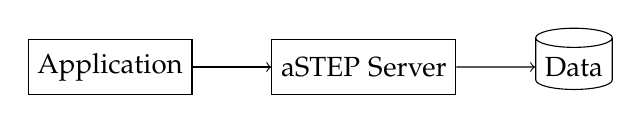
\begin{tikzpicture}[auto]
	\node[draw, minimum height=2em](Server){aSTEP Server};
	\node[draw, cylinder, shape border rotate=90, aspect=0.25, right=of Server](Data){Data};
	\node[draw, minimum height=2em, left=of Server](App){Application};

	\draw[->] (App) edge (Server) (Server) edge (Data);
\end{tikzpicture}
	\caption{The overall structure.}
	\label{fig:packageDiagramSprint1}
\end{figure}

A background service would enable the location data sampling and transfer to a server.
As seen in Figure \ref{fig:classDiagramSprint1Observer} the Observer class' main goal is to observe what activity the user is currently doing.
In Google's API for android applications this is already a feature, so this will be used.
If the activity is driving, the background service starts to store the locations with the RouteBuilder class.
Locations are also a part of Google's API and includes longitude, latitude and a time stamp.
When the Observer detects that the user stops driving, the Observer sends the route to the server.

\begin{figure}[h]
	\centering
	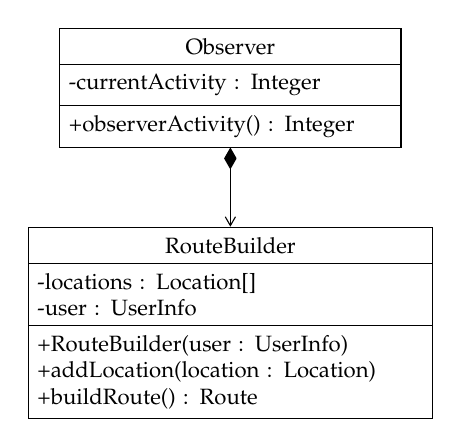
\begin{tikzpicture}[auto]
	\node[class](Observer){Observer
		\nodepart[align=left, text width=4.1cm]{two}
		-currentActivity : Integer
		\nodepart[align=left, text width=4.1cm]{three}
		+observerActivity() : Integer};
	\node[class, below=of Observer](RouteBuilder){RouteBuilder
		\nodepart[align=left, text width=4.9cm]{two}
		-locations : Location[]\\
		-user : UserInfo
		\nodepart[align=left, text width=4.9cm]{three}
		+RouteBuilder(user : UserInfo)\\
		+addLocation(location : Location)\\
		+buildRoute() : Route};
	\draw[aggregation] (Observer) -- (RouteBuilder);
\end{tikzpicture}
	\caption{The small process which should run at all time to build the routes.}
	\label{fig:classDiagramSprint1Observer}
\end{figure}


% The aSTEP core
On the server, the route is stored in a database and accessed by the RouteStabilityAnalyser.
This analyzer takes the route and compares it to other routes by the same user, to determine whether this route is a regular occurrence, and hence a stable route.

If the RouteStabilityAnalyser determines that the route is stable, the information is stored in the database with when this route is expected to occur.
The server then uses the RouteSimilarityAnalyser to find matches for the new \todo{does not need to be a new stable route??} StableRoute.
The matches are stored and new matches are transmitted to the appropriate devices to inform the users of a new match.

\begin{figure}[h]
	\centering
	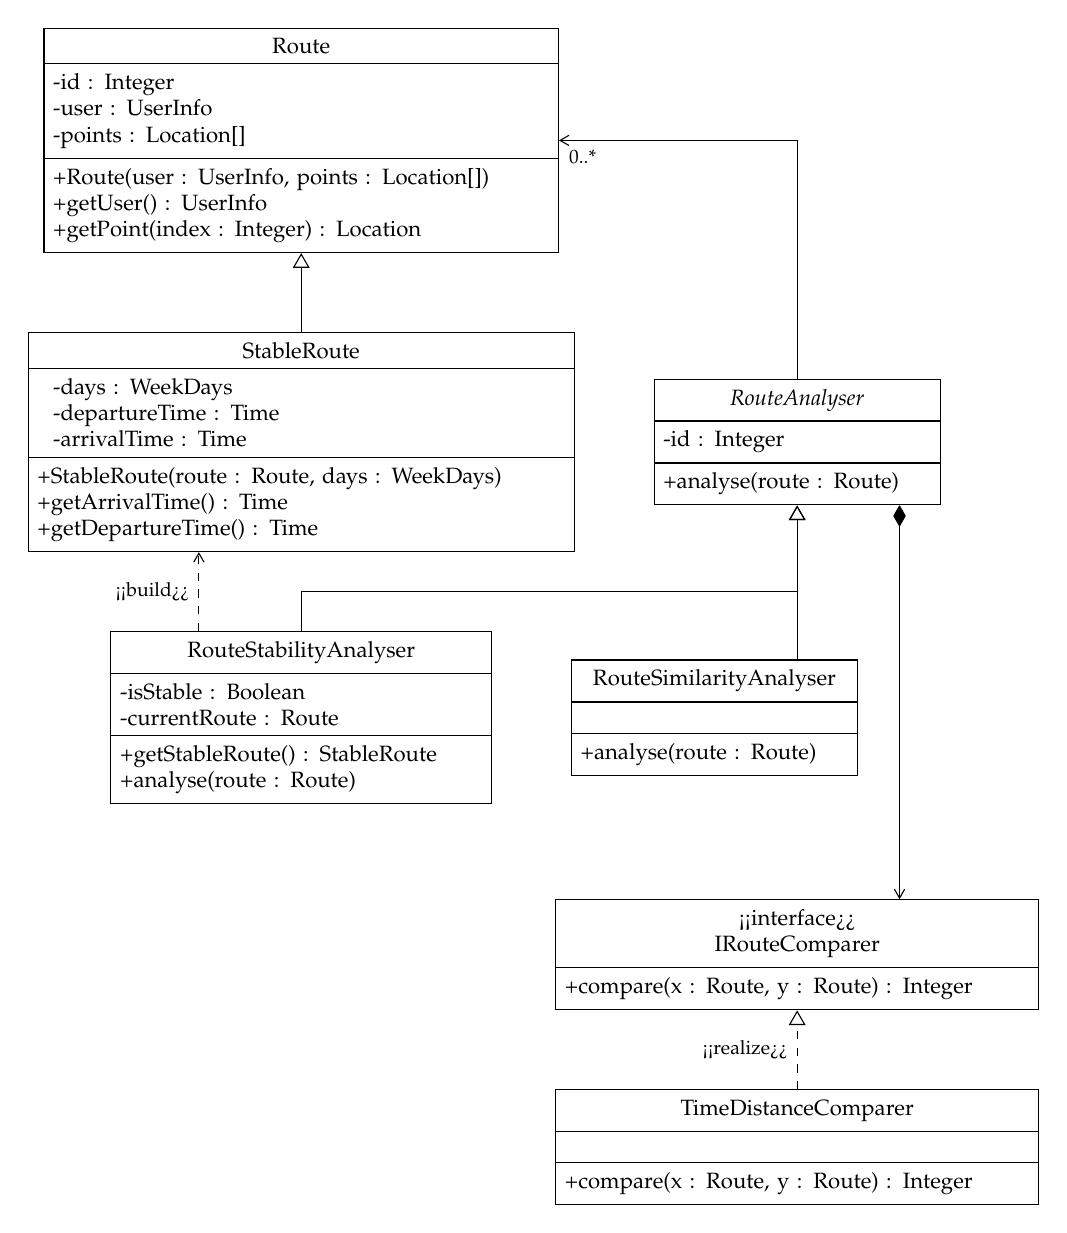
\begin{tikzpicture}[auto]
	\node[class](Route){Route 
		\nodepart[align=left, text width=6.3cm]{two}
			-id : Integer\\
			-user : UserInfo\\
			-points : Location[]
		\nodepart[align=left, text width=6.3cm]{three}
			+Route(user : UserInfo, points : Location[])\\
			+getUser() : UserInfo\\
			+getPoint(index : Integer) : Location};
	\node[class, below=of Route](StableRoute){StableRoute
		\nodepart[align=left, text width=6.3cm]{two}
			-days : WeekDays\\
			-departureTime : Time\\
			-arrivalTime : Time
		\nodepart[align=left, text width=6.7cm]{three}
			+StableRoute(route : Route, days : WeekDays)\\
			+getArrivalTime() : Time\\
			+getDepartureTime() : Time};
	\node[class, below=of StableRoute](RouteStabilityAnalyser){RouteStabilityAnalyser
		\nodepart[align=left, text width=4.6cm]{two}
			-isStable : Boolean\\
			-currentRoute : Route
		\nodepart[align=left, text width=4.6cm]{three}
			+getStableRoute() : StableRoute\\
			+analyse(route : Route)};
	\node[class, right=of StableRoute](RouteAnalyser){\textit{RouteAnalyser}
		\nodepart[align=left, text width=3.4cm]{two}
			-id : Integer
		\nodepart[align=left, text width=3.4cm]{three}
			+analyse(route : Route)};
	\node[class, right=of RouteStabilityAnalyser](RouteSimilarityAnalyser){RouteSimilarityAnalyser
		\nodepart[align=left, text width=3.4cm]{three}
			+analyse(route : Route)};
	\node[interface, below=5 cm of RouteAnalyser](RouteComparer){
		\nodepart[align=center, text width=4cm]{one}
		<<interface>>\\
		IRouteComparer
		\nodepart[align=left, text width=5.9cm]{two}
			+compare(x : Route, y : Route) : Integer};
	\node[class, below=of RouteComparer](TimeDistanceComparer){TimeDistanceComparer
		\nodepart[align=left, text width=5.9cm]{three}
			+compare(x : Route, y : Route) : Integer};

	\draw[aggregation,transform canvas={xshift=1.3cm}] (RouteAnalyser) -- (RouteComparer);
	\draw[association, dashed,transform canvas={xshift=-1.3cm}] (RouteStabilityAnalyser) -- node[label]{<<build>>} (StableRoute);

	\draw[generalization] (StableRoute) -- (Route);
	\draw[generalization] (RouteStabilityAnalyser.north) -- ++(0,0.5) -| (RouteAnalyser);
	\draw[generalization] (RouteSimilarityAnalyser.north) -| (RouteAnalyser);
	\draw[generalization, dashed] (TimeDistanceComparer) -- node[label]{<<realize>>} (RouteComparer);
	\draw[association] (RouteAnalyser) |- node[label, at end, xshift=0.3cm]{0..*} (Route.east);
\end{tikzpicture}
	\caption{The structure of the system inside the server. This package should be an isolated system within the server.}
	\label{fig:classDiagramSprint1Server}
\end{figure}\todo{fix: "This package should be an isolated system within the server."}

The application acts as an interface to the background process for the user.
This is where the user logs in and can see an overview of candidates for car pooling.

\begin{figure}[h]
	\centering
	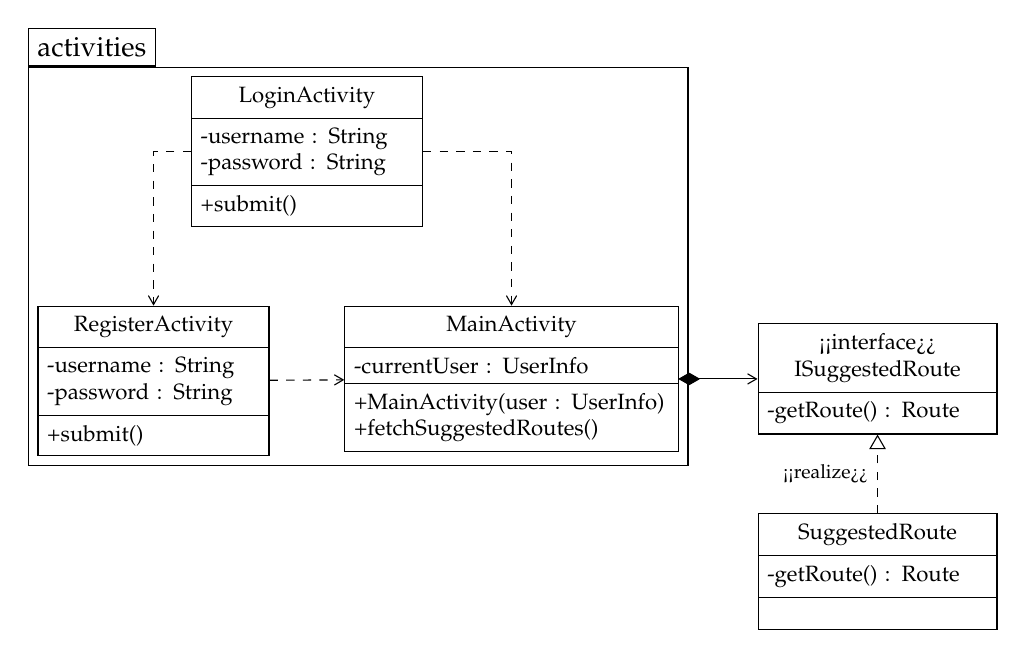
\begin{tikzpicture}[auto]
	\node[class](LoginActivity){LoginActivity
		\nodepart[align=left, text width=2.7cm]{two}
			-username : String\\
			-password : String
		\nodepart[align=left, text width=2.7cm]{three}
			+submit()};
	\node[class, below left=1 and -1 of LoginActivity](RegisterActivity){RegisterActivity
		\nodepart[align=left, text width=2.7cm]{two}
			-username : String\\
			-password : String
		\nodepart[align=left, text width=2.7cm]{three}
			+submit()};
	\node[class, below right=1 and -1 of LoginActivity](MainActivity){MainActivity
		\nodepart[align=left, text width=4cm]{two}
			-currentUser : UserInfo
		\nodepart[align=left, text width=4cm]{three}
			+MainActivity(user : UserInfo)\\
			+fetchSuggestedRoutes()};
	\node[interface, right=of MainActivity](ISuggestedRoute){
		\nodepart[align=center, text width=2.8cm]{one}
			<<interface>>\\
			ISuggestedRoute
		\nodepart[align=left, text width=2.8cm]{two}
			-getRoute() : Route};
	\node[class, below=of ISuggestedRoute](SuggestedRoute){SuggestedRoute
		\nodepart[align=left, text width=2.8cm]{two}
			-getRoute() : Route};

	\draw[association, dashed] (LoginActivity) -| (MainActivity);
	\draw[association, dashed] (LoginActivity) -| (RegisterActivity);
	\draw[association, dashed] (RegisterActivity) -- (MainActivity);
	\draw[generalization, dashed] (SuggestedRoute) -- node[label] {<<realize>>} (ISuggestedRoute);
	\draw[aggregation](MainActivity)--(ISuggestedRoute);

	\node[draw, fit=(MainActivity) (LoginActivity) (RegisterActivity)](PackageBody){};
	\node[draw, above right] at(PackageBody.north west){activities};
\end{tikzpicture}
	\caption{The class structure of the application.}
	\label{fig:classDiagramSprint1Application}
\end{figure}

This is the start of a project that will be further developed upon and expanded in the future, emphasizing the importance of reusing the server, to reduce the amount of specialized server resources.
By isolating parts that are specific to the rideshare app on the server, most of this system would be reusable.
The best example of this is the RouteAnalyser from Figure \ref{fig:classDiagramSprint1Server}.
The RouteAnalyzer filter routes according to its concrete implementation.
After the filtering, the RouteAnalyser uses the strategy pattern to determine how to compare the routes.
This enables other projects to develop their own filters and comparison functions in later projects.

To reduce the search space, a weekly stability was decided upon. \todo{did we?}
This means that the RouteStabilityAnalyser can be limited to analyze one to two months of data.
This will be further tested and evaluated in another chapter. \todo{reference to test and evaluation}\todo{add arguments}

\subsection{User Interface Design}
% General Introduction to UI - what + why
The user interface (UI) provides interaction methods between the user and the app.
As the priority of this project is functionality with regards to data collection and route generation and comparison, the UI will not be developed together with users, nor allocated excessive resources. 
The UI is developed for practical purposes, like testing, and to lay the basis for further development, but is still held to some standard which will be documented in the following text. 

\subsubsection{Design language}
% Definition
The design language is the general look and appearance of a system.
This is the foundation for the impressions and feels of the user, and affects the user experience.
The design language is selected in collaboration with another aSTEP project group, SW604F16.

% Goals
The user interface is designed to achieve the following usability characteristics \cite{DIS2014}:
\begin{itemize}
	\item Learnability
	\item Utility
	\item Safety
	\item Effectiveness
\end{itemize}

% Material design
The UI is designed to comply with the Google's Material design guidelines \cite{materialDesign}, being ``\textit{bold, graphic, intentional}''. 
Some of the Material design properties are stated in the following list, compiled of citations from the design guidelines \cite{materialProperties}:

\begin{enumerate}
	\item Material has varying x \& y dimensions (measured in dp) and a uniform thickness (1dp).
	\item Material casts shadows. Shadows result naturally from the relative elevation (z-position) between material elements.
	\item Content is displayed on material, in any shape and color. Content does not add thickness to material.
	\item Input events cannot pass through material.
	\item Material cannot pass through other material. For example, one sheet of material cannot pass through another sheet of material when changing elevation.
	\item Material grows and shrinks only along its plane.
	\item Material never bends or folds.
	\item Material can be spontaneously generated or destroyed anywhere in the environment.
\end{enumerate} 

% Paragraph regarding selection of material
Adhering the material design guidelines makes the app achieve a similar aesthetic and usage method as other apps in the Android eco-system. 
The design language aims to make the interface clean and simple, regarding colors and input methods.

\subsubsection{User interface}
% Actions in UI and design thereof
The design drafts in Figure \ref{fig:GUI-firstrun} reflect the necessary functions and the previously described design language. 

% Login and registering pages design
As the user needs a user profile in the aSTEP system to use the app, the users must be able to login if they already have a user profile, or create a new user profile.

\begin{figure}[h!]
	 \centering
	 \begin{subfigure}[b]{0.3\textwidth}
	 	\includegraphics[width=\textwidth]{figures/GUI-front.png}
	 	\caption{Login page}
	 	\label{fig:GUI-front}
	 \end{subfigure}
	 ~ %add desired spacing between images, e. g. ~, \quad, \qquad, \hfill etc. 
	 %(or a blank line to force the subfigure onto a new line)
	 \begin{subfigure}[b]{0.3\textwidth}
	 	\includegraphics[width=\textwidth]{figures/GUI-register.png}
	 	\caption{Register page}
	 	\label{fig:GUI-register}
	 \end{subfigure}
	 \caption{Draft of the login and registering pages of the app.}\label{fig:GUI-firstrun}
\end{figure}

% In-app pages design
Several views are necessary to support the different parts of the app. 
The app needs a view for login, registering, presentation of matches, and a settings screen, as can be seen in the figures in Figure \ref{fig:GUI-in-app}.

As the application must have communication to the aSTEP server, which have an requirement of registration of users, it is necessary to have a register and login screen in the application. The username will be used as a identifier for the user, and it will be used both for the aSTEP server, but also for the application it self. It will be the identifier to differ between each user, and ensure users are matched up with other users correctly when comparing routes.

The application must have a main screen, and it is chosen that should be the route match list. On this screen the user will be presented a list of other users, which most likely is a good match. The users listed should be in an descending order, with the highest rated match at the top. A short description about the users and match should be displayed, such as the users full name, phone number, the match score, and what day of the week the user drive the relevant route.

A settings screen is needed because the users should have the option to change there initial information from when they registered. The settings screen also server as a screen where users can specify their preferences. Such information is, wherever the users have a car with X numbers of seats and if the users is looking for, or giving a lift.
In addition should there exist a navigation drawer from where the user can navigate around the application.

\begin{figure}[h!]
	\centering
	\begin{subfigure}[b]{0.3\textwidth}
		\includegraphics[width=\textwidth]{figures/GUI-main.png}
		\caption{Main page}
		\label{fig:GUI-main}
	\end{subfigure}
	~ %add desired spacing between images, e. g. ~, \quad, \qquad, \hfill etc. 
	%(or a blank line to force the subfigure onto a new line)
	\begin{subfigure}[b]{0.3\textwidth}
		\includegraphics[width=\textwidth]{figures/GUI-settings.png}
		\caption{Settings page}
		\label{fig:GUI-settings}
	\end{subfigure}
	\caption{Draft of the views in the app.}\label{fig:GUI-in-app}
\end{figure}


%\section{Implementation}

\subsection{Location Gathering Background service}
% metatext
This subsection will describe the contents of the implementation of the background location gathering.
The new implementation is based on the poor results of the location gathering method implemented in sprint 2 that was not working as intended.
The code examples in this section will not include potential logging and debugging lines as to save space and they do not influence the functionality of the code.


% activityRecognitionInstantiation
The location gathering should first detect that the device is in a driving activity and then begin recording locations, according to the design described in the design section.
To achieve the functionality, the app must connect to a Google API client and subscribe to activity recognition.
The subscription to the activity recognition is shown in Listing \ref{activityRecognitionInstantiation}.
The activity recognition can thereafter check that the detected activity is a driving activity, and accordingly activate the location gathering.

\begin{lstlisting}[language=Java, label=activityRecognitionInstantiation, caption=Initialization of activity recognition.]
if(activityDetectionBroadcastReceiver == null) {
	activityDetectionBroadcastReceiver = new ActivityDetectionBroadcastReceiver(googleApiClient, this);
	LocalBroadcastManager.getInstance(this).registerReceiver(activityDetectionBroadcastReceiver, new IntentFilter("fapptory_inc.rideshare.BROADCAST_ACTION"));
}
\end{lstlisting}

The \texttt{activityDetectionBroadcastReceiver} is instantiation of the\\ \texttt{ActivityDetectionBroadcastReceiver} class, utilizing the \texttt{googleApiClient} and the \texttt{MainActivity}.

The broadcast receiver is then applied by registering to the \gls{rs} app's\\ \texttt{BROADCAST\_ACTION}, so that the \texttt{activityDetectionBroadcastReceiver} only handles broadcasts sent by \gls{rs} and not by other apps.

% ActivityIntentService broadcast description



% Activity Detection Broadcast Receiver
The main operations in regards to activity detection and location gathering are done by the activity detection broadcast receiver.

When the \texttt{activityDetectionBroadcastReceiver} receives a RideShare broadcast, the extra data in the broadcast is stored in the \texttt{ArrayList<DetectedActivity> detectedActivities}.
The \texttt{detectedActivities} is iterated over, shown in Listing \ref{activityRecognitionIteration} to find the driving activity \texttt{DetectedActivity.IN\_VEHICLE}.
The \texttt{startLocationUpdates()}, which is described later, is called if the confidence is above the threshold and if locations are not currently being recorded.
Line 8 controls the location cache in case a drive is stopped temporarily and starts again, appending the cached route to the actual route.

\begin{lstlisting}[language=Java, label=activityRecognitionIteration, caption=Iteration over received list of activity recognition.]
for (DetectedActivity da: detectedActivities){
	if(da.getType() == DetectedActivity.IN_VEHICLE){
		if(da.getConfidence() >= ACTIVITY_CONFIDENCE_VALUE){
			if(!isCurrentlyCollectingLocations) {
				startLocationUpdates();
				isCurrentlyCollectingLocations = true;
			}
			if(potentialStopDrivingActivity && potentialAstepRoute.size() > 0){
				astepRoute.addAll(astepRoute.size(), potentialAstepRoute);
				potentialAstepRoute.clear();
			}
			lastDetectedVehicleActivity = System.currentTimeMillis();
			potentialStopDrivingActivity = false;
			drivingActivityDetected = true;
		}
	}
}
\end{lstlisting}

% Location Updates Request
The \texttt{startLocationUpdates()}, shown in Listing \ref{startLocationUpdates}, is called to gather locations regularly.
It checks for individual permission for fine location access, as required by Android M (SDK level 23 and higher), before requesting location updates from the Google Play Services' \texttt{LocationServices}.
The location updates request is based on the Google API client instantiated in \texttt{MainActivity} and a \texttt{locationRequest}.
The \texttt{locationRequest} is defined with properties regarding location update interval, fastest interval, and location quality priority, respectively set to \todo{agree upon constants} 60 seconds, 120 seconds and \texttt{PRIORITY\_HIGH\_ACCURACY}.

\begin{lstlisting}[language=Java, label=startLocationUpdates, caption=Start location updates functions.]
public void startLocationUpdates(){
	// Check individual permissions for Android M (SDK level 23) and up.
	if(Build.VERSION.SDK_INT >= 23) {// Android M permission check
		if (ActivityCompat.checkSelfPermission(mainContext, 			Manifest.permission.ACCESS_FINE_LOCATION) == PackageManager.PERMISSION_GRANTED){
			// Initialize location request, where updates are received by onLocationChanged()
			LocationServices.FusedLocationApi.requestLocationUpdates(googleApiClient, locationRequest, this);
		}
	}else { // Without individual permission tests: Initialize location request, where updates are received by onLocationChanged()
	LocationServices.FusedLocationApi.requestLocationUpdates(googleApiClient, locationRequest, this);
	}
}
\end{lstlisting}

To send the routes gathered through the location service, the communication with \gls{astep} must be established.

\subsection{App-to-aSTEP communication}
% ja..
%\section{Test}
A test of the location gathering background service was performed to examine the functionality, performance and reliability.

\subsection{Location gathering as background service}
% test setup
The \gls{rs} app was built and installed on three units to test on a variation of devices.
The devices were a Sony Xperia Z2, a Samsung Galaxy S6 and a Huawei Nexus 6P, all with Android Marshmallow 6.0.1 as operating system.
The app was opened and the necessary permissions were granted, so that the app could function properly.
The app was configured with the values seen in Table \ref{tab:appconfig}.

\begin{table}[!ht]
	\centering
	\begin{tabular}{l r l}
		Variable description & Value & Unit\\
		\hline
		Fastest location update interval & 60000 & milliseconds\\
		Target location update interval & 60000 & milliseconds\\ 
		Activity confidence value & 80 & percent\\
		Activity stop threshold & 180000 & milliseconds\\
		Minimum number of route locations & 4 & locations \\
		Request activity updates & 5000 & milliseconds\\ 
	\end{tabular}
	\caption{Parameter configuration in test of the background service route tracking.}
	\label{tab:appconfig}
\end{table}

% device setup
\iffalse
To make sure the app would gather locations in different states, the phones had different configurations.
The Xperia Z2 was locked and connected to a computer for debugging purposes and logging events.
The Nexus 6P had the app open with a locked and turned off screen. 
The Galaxy S6 had the app opened, was returned to the home screen and then locked.\todo{not sure if this paragraph is necessary}
\fi
% route plan
The route driven to test the location gathering can be seen in Figure \ref{fig:testroute}.
The route was driven with the intention of gathering the whole route as a single route on each of the devices.
The drive had one stop at the point marked by a green square in Figure \ref{fig:testroute}.
The stop had a duration of 2 minutes, thus not passing the threshold value of 3 minutes.
The drive continued and ended at the start position, where the persons of the respective devices walked from the vehicle to the group room.

\begin{figure}[h]
	\begin{subfigure}[b]{0.55\textwidth}
		\includegraphics[width=\textwidth, trim={0 0 1cm 0},clip]{figures/testroute.png}
		\caption{Test drive route, driven clockwise from the red pin.}
		\label{fig:testroute}
	\end{subfigure}
	\begin{subfigure}[b]{0.44\textwidth}
		\includegraphics[width=\textwidth, trim={0 0 2cm 1.2cm},clip]{figures/testRouteRecordings.png}
		\caption{Recorded routes. Orange route is Nexus 6P, red route is Xperia Z2 and green route is Galaxy S6.}
		\label{fig:testrouterecordings}
	\end{subfigure}
	\caption{Actual route and recorded route data.}
\end{figure}

% test results
All three devices were able to gather the driven route. 
The routes were recorded with approximately the same start and end time, and the recorded routes can be seen in Figure \ref{fig:testrouterecordings}. 
As the figure shows, the gathered route data relatively accurately represent the actual route.


The Xperia device had the largest deviation from the actual route, and this could be caused by multiple factors.
Because the device was placed below the debugging laptop, interference with the GPS signals could occur.
The device could also have a poorly manufactured GPS unit.
This is not further investigated, as the two other devices gathered fairly accurate locations during the test.



% results evaluation
The test reveals that the app is able to gather locations whilst the app is not actively being utilized by a user.
The location accuracy seems to be device specific.
Location gathering as a background service is considered accomplished and the respective requirement is evaluated as fulfilled.



\subsection{Route Match Algorithm}\label{sec:s3algtest}
% metatext
The route matching algorithm is implemented by one of the \gls{astep} outdoor groups, and to check that the implementation reflects the intention a test is performed.

The implementation is tested with a sequence of routes inserted into a previous empty route database.
By adding routes sequentially, we can anticipate the matching outcome for each addition.


% test data
\textbf{Test Data}\\
A number of cases should be tested, and we generate route data for each. 
Before the route data is input users U1, U2, U3 and U4 are created to the \gls{astep} system.

First, the stable route generation must be confirmed functioning.
A route is created for U1 and made two copies that were slightly edited in location and time, and skewed respectively one and two weeks ahead of the original route.
These three routes should be assessed a high matching score, close to 1, and be considered a stable route for this user.

Second, the algorithm should not be matching routes that are not relevant in location or time.
U2 gets two routes added not matching in location, as seen in Figure \ref{fig:algroutes}.
The blue U2 route is during the day time and the black during night time.
These routes should thus be assessed a low match score, assumed 0.

Because the algorithm should match routes of different users, we thirdly created two routes for the user U3.
The routes were differencing slightly in locations and time, but were made with the intention to match with each other, with one week difference in time.
The routes were also made to roughly overlap with the routes of U1, so that U1's stable route would roughly be a sub-route of the U3 route.

Lastly, the U4 route was made to discern location and time matching of the algorithm.
The route is stable and approximately at the same time as the U1 and U3 routes, but is directed in the opposite way, northwest instead of southeast.
The U4 route should match poorly with U1 and U3 routes, close to 0, but could score a bit higher, as the locations overlap with U3 route.

\begin{figure}[h]
	\centering
	\includegraphics[width=0.7\textwidth]{figures/algorithmroutes.png}
	\caption{Generated routes to be tested by the algorithm.}
	\label{fig:algroutes}
\end{figure}


% other group executed their implemenation on test data
\textbf{Test Execution}\\
We had no influence over the actual method of the testing, but we received the following test results in Figure \ref{fig:algresults} from the outdoor group.


% test results
\textbf{Test Results}\\
The test results seen in Figure \ref{fig:algresults} reveal that the algorithm is performing correctly.
The results correspond to the assumptions made during the data generation.
All three routes of U1 are matched highly, as expected.
The U3 route is matching reasonably well with the U1 routes, and neither of the U1 routes are matching with the U3 route.
The results reflect that U3 can pick up U1 along the way, while U1 will have to make a significant detour to pick up U3.

\begin{figure}[h]
	\centering
	\includegraphics[width=0.8\textwidth]{figures/newtestresultrs.png}
	\caption{Results generated by the implemented algorithm.}
	\label{fig:algresults}
\end{figure}


% test results conciderations 
\textbf{Test Conclusion}\\
The algorithm test results are considered sufficient for the current application. 
However testing, including user interviews, over large amounts of data for actual users is necessary to confirm the practical convenience of the score results.
The design of the algorithm allows adjustment of several parameter concerning distance, time and the the weight of those in the final score by changing parameters in the \gls{rs} server's call to \gls{astep} system. 


% Sprint 2
\chapter{Sprint 2}
Whereas the main topic of sprint 1 was an overall analysis and collaboration agreement, the topic of sprint 2 is design and development based on the results of sprint 1. The sprint intentions are to develop a route comparison algorithm that can be implemented in the aSTEP system, and to develop an app that has basic functionality, to be advanced and improved upon in sprint 3.

This chapter contains documentation of the analysis, design, implementation and test phases of the algorithm and app development performed in sprint 2.
\section{Analysis}
This section contains the analysis of app functionality, Android app development, \gls{rs} algorithms and communication with the aSTEP system.

%temporary title
\subsection{App functionality}
% meta shit
The app user interface is a low priority task during this project.
However, the app needs basic functionality, according to the requirements.

% User management
To be able to separate different routes, and to assign them to their respective users, there has to be a user management system, so that each user has its own ID.

% Ride matches
The user should also be informed with relevant information of ride matches, so that the user can make a decision of sharing a ride or not.

% User settings
The user of the application should also be able to adjust their settings.
The settings are preferences regarding different properties of ride sharing.
The user should be able to decide if it wants to get a ride or give a ride or both.
There are also properties of the user itself, like a description and a picture, that other users can access to decide if they want to share a ride with the named user.



% other shit...



\subsection{Android Development Platform}
When developing Android applications one of the first choices to consider is which API levels to target \cite{usesSDK}.
The ``\textit{API Level is an integer value that uniquely identifies the framework API revision offered by a version of the Android platform.}'' according to Android Developers \cite{usesSDK}.
The distribution of the Android version levels are shown in \ref{fig:dashboard}.

``\textit{The manifest file presents essential information about your app to the Android system, information the system must have before it can run any of the app's code.}'', according to Android Developers \cite{androidManifest}.
The manifest requires to specify the API level for three definitions: minimum, target and maximum. 
The target and max versions requires few consideration to determine.
The ``targetSdkVersion'' reflects the version to which the app is developed and tested against, without enabling compatibility behaviors.
The ``maxSdkVersion'' reflects the highest API level that an app is designed to run.
Both of these are set to the highest API level available during the start of the development, which is API version 23.

\begin{figure}[h!]
	\centering
	\includegraphics[width=0.7\textwidth]{figures/android-chart-march.png}
	\caption{Android version distribution, March 2016 \cite{androidDashboard}}
	\label{fig:dashboard}
\end{figure}

The last API level which needs to be specified is the ``minSdkVersion''.
This entry specifies the lowest API level which an app supports.
A cause of this is that every device with an API level lower than the specified minSdkVersion will not be compatible with the app.
Supporting older API versions requires development efforts, typically implementing functionality though the Android Support Library \cite{androidSL}.
For this project we choose to target a higher API level for to simplify the development process.
At the time of writing, the platform version distribution sum of API levels greater than or equal to 21 (Android Lollipop) is 35,3\%.
API version 21 is chosen as the minSdkVerison, the main reason for this choice is to minimize development time for user interface, as API level 21 added support for Android's new material design style \cite{android5API}. Refraining from further backwards compatibility allows the project focus to be on the functionality of the app. 

\subsection{Periodic Tasks}\label{ssec:periodictasks}

When the app is installed the program needs to run a task periodically to cache locations.
\Citet{friesen2015android} writes about how this can be done in the Android API with the AlarmManager and the JobSchedular.

\paragraph{AlarmManager}
In the first Android version (API 1) the AlarmManager was created to handle alarms.
They implemented it as a general class which can call any task after a given period has passed.
The alarm can then be set to be reoccuring which means that we can use this to cache location data in a set interval.

\paragraph{JobSchedular}
In Android 5.0 (API 21) an alternative to the AlarmManager was implemented, the JobSchedular.
This functions in a similar way as the AlarmManager, but tries to bach the jobs together and fire them at the same time.
This means that the device can save power by avoiding going to sleep just to wake a short moment later.
The sacrefice is precision. 
While the AlarmManager has the option to occur at a exact time, the JobSchedular does not.
This is needed to give the AlarmManager enough control to effeciently bach the jobs together.

\todo{Something is missing} Because the timing of the location data is less important than the constant stream of data the JobSchedular.
This has the advantages of saving power making it more likely that the device will stay powered for the duration of the trip.
And by extention giving a complete route.

% algorithm analysis if necessary
\subsection{Algorithms for ridesharing}


% aSTEP system functionality analysis: communication with aSTEP
\subsection{Communication with aSTEP}\label{ssec:communicationwithastep}
% meta
To be able to utilize the aSTEP system, the communication protocol and functions must be analyzed. 
The analysis is based on the current development and planning of the API and other functions.

% aSTEP organization - groups
The status and intended functions are established in collaboration with the other project groups responsible for the aSTEP system side of the development. 
The main groups we are involved with are the user management group and outdoor location based services groups.

% What does the aSTEP system look like?
The design of the aSTEP system at this point is consisting of an API that apps and services can communicate with, and a backend with user management and location based services, which is stored in a database system.
However, the only relevant part for the \gls{rs} solution for us is the API, as the lower level of the aSTEP core is administrated by other groups.

% What is stored in aSTEP
The aSTEP system will store information regarding location data, and basic user information. 
The data stored in the aSTEP system, relevant to this project solution, is:
\begin{itemize}
	\item Location data consisting of userID, routeID, a set of GPS coordinates and timestamp.
	\item Username
	\item Password
\end{itemize}

The aSTEP user management system does not provide storage of data regarding contact information for aSTEP users.
The only information stored is a username and password to keep the aSTEP core as simple as possible.
Additional information that is required to make the app work as intended is each of the app groups own responsibility.
The aSTEP users is made to ensure the correct permissions is giving to the correct user, to ensure the appropriate data is returned to each user.
An API call can not be done without the user first being authenticated with a valid login.

% How to cummunicate with aSTEP
The communication with aSTEP is done through a REST API over Hypertext Transfer Protocol, decided in agreement between the aSTEP project groups.
REST is an abbreviation of REpresentational State Transfer, and is a communications design often used in for HTTP-communication\cite{REST}.
Accordingly, the communication is performed by making queries to the aSTEP system. 
All communication must be done as a request from the device, where the aSTEP server then will respond.


% api functions
At the current stage of the development of aSTEP, the following API functions are available form user management and location services:
\begin{table}[]
	\centering
	\begin{tabular}{ll}
		LBS & UM    \\
		\hline
		\begin{tabular}[t]{@{}l@{}}
			GetAllEntitiesInArea\\ GetAllEntitiesInTimePeriod\\ GetAllGroupMemebersLocationAndName\\ GetAllFriendsInArea\\ GetAllFriendsInRadius\\ GetAllGroupMembersInArea\\ GetAllGroupMembersInRadius\\ PostLocationData\end{tabular}
		&
		\begin{tabular}[t]{@{}l@{}}
			Create user\\ Get token\\ Update password\\ Edit privacy settings\\ Allow user2 to access user1's info\end{tabular}
	\end{tabular}
	\caption{Currently planned aSTEP API functions.}
	\label{tab:sprint2-api}
\end{table}
\todo{reference this table. Add information about the functions.}

When using the aSTEP API it should be ensure to use the correct calls in the right way.
The API is providing a POST-request under the name ``PostLocationDat'', as listed in \ref{tab:sprint2-api}, which is the method to use when sending location data to the aSTEP core.
When using this POST it is important to ensure the correct parameters is used.
The call will accept location data as an coordinate consisting of longitude and latitude, a precision value, and a value representing time of day in milliseconds.

% Sprint 2 krav
\subsection{Requirements for the second sprint}
%meta
Sprint two is the first of the two middle sprints that have implementation as the primary focus. In this section, the main issues to be solved in the current iteration will be presented.

% algorithm
\textbf{Route Matching Algorithm}\\
In this sprint, the algorithm for comparing routes must be researched and developed. 
It should be developed to an extent so that it is constructed as pseudocode of the algorithm, to be handed over to another \gls{astep} group, and be implemented in the \gls{astep} system.

\textbf{User Data}\\
User information such as username, password, and login token, must be analyzed to figure out where this information should be stored, and how it should be handled regarding communication between the application and the aSTEP server. 

\textbf{RideShare app}\\
A base for the functionalities for the \gls{rs} application should be implemented. 
The implementation should include a working \todo{?} including of the Google Play Services and the application should be able to collect and store location data. 
The application should also have functionality to run as a background services, so that location data can be collected at all times.

\textbf{System Architecture and Communication}\\
Communication between the \gls{rs} application and \gls{astep} server should also be researched and an implementation of the communication should be initialized in this iteration, ensuring the next iteration will have a base for communication. 
It should be considered how to handle storing the collected location data and how much should be stored where, either on the device or on the \gls{astep} server.

\textbf{Mock Data}\\
If there is spare time during the sprint, it should be considered to acquire mock up location data related to mock up users. 
This data could be used in the third iteration to test if the algorithm works as intended.
\section{Design}

% metatext
This section contains documentation of the design of the rideshare solution.
The parts to be designed in this sprint are the overall system design, reflecting the changes in the aSTEP system, and the algorithms to generate stable routes and route matches.

% System design
\subsection{System design}
% metatext & redesign motivation
In the first iteration, the \gls{rs} system was designed to consist of two parts: The \gls{rs} app and the \gls{astep} system.
Because the \gls{astep} does not provide the anticipated services, such as storing basic user information\todo{?}, this data must be stored elsewhere.
This forces a redesign of the system.
This section contains descriptions of the redesign of the different parts, and a definition of their respective responsibilities.


% data conciderations
The \gls{astep} system still provides the functionality to store locations and route history for users.
The \gls{rs} app continues to collect \todo{smt missing?} device location data.  
The \gls{rs} solution will need additional data storage to fulfill the defined system requirements, because the \gls{rs} users need to be able to contact each other, to make the \gls{rs} app usable\todo{try to change the structure of this this sencente}.


% btw, an RSS can be used for more! Match scores, etc.
The \gls{astep} system is supposed to be kept as generalized and modular as possible, and when combined with the lacking user information storage, app specific data could also be stored together with the user information.
The app specific data is information, such as match scores between routes.


% solution alternatives
A solution that we regards as appropriate for the task is using a custom solution server, to utilize together with the \gls{rs} app and \gls{astep} system.
The \gls{rs} server could store the extra user data and connect the user to the \gls{astep} user ID, so that each \gls{rs} solution user has a unique \gls{astep} user, with contact information stored on the \gls{rs} server.


% instanciate RSS (RideShare Server)
The \gls{rs} server has two main purposes.
Firstly, to store additional information about the system users, and secondly to store the score \todo{} for previously assessed scores \todo{} between given stable routes.
The different purposes and responsibilities of the parts depicted in Figure \ref{fig:s2systemdesign} will be elaborated in the following text.


% app responsibilities
The \gls{rs} application continues to be responsible for the interaction with the user as well as collecting the location data needed to track routes and recommend ride partners.
The app communicates with both the \gls{rs} server and the \gls{astep} server through their respective API's.


% user management responsibilities <--um@rss or um@astep?
The API and server associated with the \gls{astep} system will be responsible for saving and retrieving location and route data for each user in the system.
The \gls{astep} system is also responsible for the basic user profile, consisting of a userID and a password.
A user profile is used to identify location data, and to store other users' permissions to access the actual user's location data.
The \gls{rs} server will be used to store additional information regarding users and routes.
The user information that will be stored, is the additional contact information.

\begin{figure}[!h]
	\centering
	\includegraphics[width=\textwidth]{figures/SystemDesign.png}
	\caption{System design, including all major parts of the solution.}
	\label{fig:s2systemdesign}
\end{figure}


%This means that a user will be represented in the \gls{rs} solution and in the \gls{astep} system. 


% Definition of RIDESHARE(TM) server responsibilities
Beyond storing scores for route matches and additional user info the \gls{rs} server will also be responsibly for sending request to the \gls{astep} server, concerning calculations about stable routes and route matches.
To be able to gain access to each user's location data from \gls{astep}, the \gls{rs} server has to store some sort of login information.
The \gls{astep} system provides a login token, so that a password does not need to be stored on the \gls{rs} server.


% Completed system design
The final system design developed in the second iteration, described in this section, can be seen in Figure \ref{fig:s2systemdesign}.



% Algorithm
\subsection{Algorithm}
The system uses a custom developed algorithm to determine whether two routes are a good fit.
This algorithm is loosely based on a simplified version of \citet{ghoseiri2011real}, with regards to the process of the evaluation of a match.
In the paper, the algorithm considers multiple aspects when assessing matches, such as smoking, gender and age preferences.
The criteria are practical to some extent, but the focus of the \gls{rs} system are the time and distance criteria.
A position is spatial-temporal, whereas a location is a spatial point and a time is a temporal point.
A route is a chronological list of positions.
A disadvantages of the algorithm presented here is that the distance is calculated as a euclidean distance rather than a map distance. 
This would be a obvious place for future improvements to the algorithm.

To illustrate how the algorithm should work for different routes an example is introduced. The example can be seen in Figure \ref{fig:algEx1}.
\begin{figure}[!ht]
    \centering
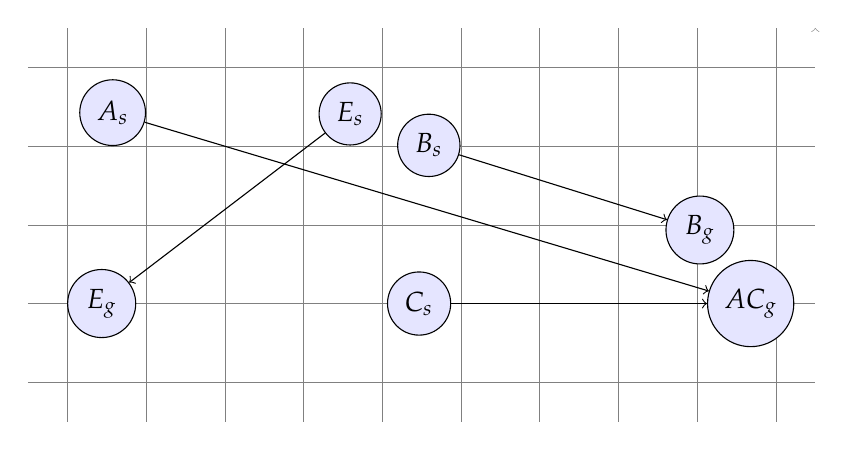
\begin{tikzpicture}[ 
		auto,
        node distance = 1 cm, 
        vertex/.style = {circle, draw, fill=blue!10}, 
        label/.style={fill=white},
        ->
    ]
    %\draw[step=0.2cm,gray,very thin] (-6,-1) grid (4,3);
    \draw[step=1cm,gray,very thin] (-6.5,-1.5) grid (3.5,3.5);

    \node[draw=none] (center){};
    \node[vertex, above left  = 2cm and 5cm of center]   (1) {$A_s$};
    \node[vertex, above left =  1.6cm and 1cm of center]   (2) {$B_s$};
    \node[vertex, right = 2cm of center]   (3) {$AC_g$};
    \node[vertex, left =     of center]   (4) {$C_s$};
    \node[vertex, above right =  0.5 cm and 1.6 cm of center]   (5) {$B_g$};
    \node[vertex, left = 5 cm of center] (6) {$E_g$};
    \node[vertex, above left = 2 cm and 2cm of center] (7) {$E_s$};

    \draw (1) -- (3);
    \draw (2) -- (5);
    \draw (4) -- (3);
    \draw (7) -- (6);

\end{tikzpicture}
    \caption{Alice, Bob, Carol and Eve's stable routes. Each grid represent a 5$\times$5 km area.}
    \label{fig:algEx1}
\end{figure}
The example introduces four users, each with one stable route in this example. In addition to the location of their routes, we also have their departure and arrival times that can be seen in Table \ref{timetable}.
\begin{table}[]
\centering
\begin{tabular}{@{}llll@{}}
\toprule
\textbf{User} & \textbf{Departure} & \textbf{Arrival} & \textbf{Distance} 	\\ \midrule
Alice         & 07:20                   & 07:55       & 36.5 km 			\\
Bob           & 07:35                   & 07:50       & 14 km  		  		\\
Carol         & 08:05                   & 08:30       & 15 km         		\\
Eve           & 07:30                   & 07:50       & 18 km         		\\ \bottomrule
\end{tabular}
\caption{The four users departure and arrival times as well as their distances.}
\label{timetable}
\end{table}

For this example, the goal will be to find out if any route matches with Alice's route $\{A_s-A_g\}$
The outcome should be a score representing if Alice, on the way through route $r$, should pick up some of the persons Bob, Carol or Eve, for each of their routes.

The expected outcome is Bob will match reasonable in both distance and time difference and hence be given a score indicating a match.
Carol is expected to match reasonable in distance as well but will lack a match comparing travel times and therefore not produce a match.
Comparing with Eve a somewhat match on time is expected while the distance will be way off.
The score represents the match of the routes of Alice and each of the other, and should be expressed as a decimal value from 0 to 1 which tells how good the match is.
0 represents a bad match, a major detour or not compatible times, and 1 represents a perfect match, and requires no detour.
A comparison will be made for $r_1$ against $r_2$.
To summarize, the algorithm takes a route $r$ and two positions to compare against; start ($s$), and goal ($g$) as arguments.
The algorithm then returns a decimal value between 0 and 1.

\subsubsection{Time Distance Analyser Algorithm}

In the algorithm, there are two aspects to be evaluated; time and distance.
These are assumed to be evaluated by two sub algorithms that both takes the route and two points as input and return a value from 0 to 1 depending on how closely they match.

If either time or distance is deemed unacceptable they are being assessed a score of 0, thus the whole match is unacceptable and given the a final score of 0.
From the scores of the sub algorithms, the final score can be expressed as the average score $\frac{d+t}{2}$, where $d$ is the distance score and $t$ is the time score.
To increase flexibility of the algorithm, two constants are introduced $d_\gamma$ and $t_\gamma$.
These constants enables weighting of the time and distance score independent of each other by expanding the expression to $\frac{d\times d_\gamma+t\times t_\gamma}{d_\gamma+t_\gamma}$.

For our example we simply set both $d_\gamma$ and $t_\gamma$ to 1. 

\begin{algorithm}
	\caption{Time Distance Analyser Pseudocode}
	\label{alg:timedistanalyser}
	\begin{algorithmic}[1]
		\Require 
		\Statex let $d_\gamma$ be the modifier for distance in $\mathbb{R}_{>0}$
		\Statex let $t_\gamma$ be the modifier for time in $\mathbb{R}_{>0}$
		\Statex 
		\Function{TimeDistanceAnalyser}{$r, s, g$}
			\State $d\gets$\Call{DistanceAnalyser}{$r, s, g$}
			\State $t\gets$\Call{TimeAnalyser}{$r, s, g$}

			\If{$d > 0 \wedge t > 0$}
				\State \Return $\frac{d\times d_\gamma+t\times t_\gamma}{d_\gamma+t_\gamma}$
			\Else
				\State\Return 0
			\EndIf
		\EndFunction
	\end{algorithmic}
\end{algorithm}

The final algorithm can be seen in Algorithm \ref{alg:timedistanalyser}.
Line 2 and 3 are calls to the algorithms that solve the subproblems of scoring the time and location, and line 4 to 8 is the logic described in the previous paragraph.

The following sections will cover the sub algorithms.
First, the distance analyser algorithm will be described, followed by the time analyser algorithm.

\subsubsection{Distance analyser}
The distance analyser algorithm takes a route and two end points and assesses the score for the detour when only considering the distance.
To do this, it is required to define how long the longest acceptable detour should be.
The algorithm also needs a way of calculating the distance between two discrete locations, which can be performed by the function for euclidean distances.
This leads to the following algorithm, where the symbol $\mathbb{L}$ is used to denote the set of all possible locations:

\begin{align*}
	dist : \mathbb{L}\times\mathbb{L} &\rightarrow \mathbb{R}_{\geq 0}\\
	a, b &\mapsto \sqrt{(a_{latitude} - b_{latitude})^2 + (a_{longitude} - b_{longitude})^2}
\end{align*}

\begin{algorithm}
	\caption{Distance Analyser pseudocode}
	\label{alg:distanalyser}
	\begin{algorithmic}[1]
		\Require 
		\Statex let $\beta$ be the largest acceptable detour length in $\mathbb{R}_{>0}$ 
		\Statex 
		\Function{DistanceAnalyser}{$r, s, g$}
			\State let $r_s$ be the closest point to $s$ in $r$
			\State let $r_g$ be the closest point to $g$ in $r$
			\State $d_s\gets dist(r_s, s)$\Comment Pickup detour distance
			\State $d_g\gets dist(r_g, g)$\Comment Set off detour distance
			\State\Return $1-\frac{d_s + d_g}{\beta}$
		\EndFunction
	\end{algorithmic}
\end{algorithm}

The distance analyser algorithm, as seen in Algorithm \ref{alg:distanalyser}, finds the points on the route that are closest to the start and end points.
From those points, the algorithm approximates the detour required to take by the driver to pick up the passenger.
The approximation assumes that the driver's new route distance will be the original length plus the distances to the passengers start point and goal point.
This assumption does not represent every detour and thus this is an area for future optimization.

The final score for the distance analyser is calculated by taking the total detour length and dividing it by the length of the largest acceptable detour.
This results in a value between 0 and 1 when the detour is less than the largest detour, and greater than one when the detour is longer.
The value is inverted by subtracting it from 1 to make greater values better matches, as required by Algorithm \ref{alg:timedistanalyser}.
If the value is greater than the acceptable detour length, the inversion in the return statement will generate a negative value, hence causing Algorithm \ref{alg:timedistanalyser} to return a result representing no match.

In the example introduced in the beginning of this chapter, the longest detour is set to be 25\% of Alice's total commute and Alice's route is modeled as the line  $y = \frac{4}{7}-\frac{2 x}{7}$.
It is assumed that Alice's route have tracking points continuously in the line, and therefore a line to point distance calculation is used in this example, this means $r_s$ and $r_g$ will be calculated simultaneously as the distance is calculated.
This gives the the results showed in Table \ref{tbl:distance} when applying the distance  Algorithm \ref{alg:distanalyser}.

\begin{table}[!ht]
\centering
\begin{tabular}{@{}llll@{}}
\toprule
\textbf{User} 	& \textbf{$d_s$} & \textbf{$d_g$} 	& \textbf{return value} 	\\ \midrule
Bob         	& 3.57 km        & 1.85 km	    	& 0.550		 			\\
Carol         	& 4.12 km        & 0 km       		& 0.609        		\\
Eve           	& 9.62 km        & 4.12 km		    & -0.505        		\\ \bottomrule
\end{tabular}
\caption{The detour distance for Alice compared to the other users as well as the score of the DistanceAnalyser for each route.}
\label{tbl:distance}
\end{table}

Table \ref{tbl:distance} presents the results for the distance analyser.
The algorithm assesses the best results for Carol, followed by Bob while Carol yields a negative result since Alice's detour becomes longer than the acceptable 25\%. 


\subsubsection{Time analyser}
The time analyser algorithm works similarly to the distance analyser algorithm. 
It is also designed to take two points and a route as input and to return a score representing the time differences.

When determining time difference two things should be taken into consideration; the detour duration and the existing differences in time.
The detour duration can be approximated by multiplying the detour distance with the time it takes to travel a distance unit.

Each position in each driver's route has a timestamp for when the location was visited.
This can be used to determine the relative time distance between two points by using the following function:
\begin{align*}
	time : \mathbb{L}\times\mathbb{L} &\rightarrow \mathbb{R}_{\geq 0}\\
	a, b &\mapsto | a_{time} - b_{time} |
\end{align*}

The calculated detour time and relative time difference enables an approximation of the inconvenience the ridesharing is for the participants in the potential match.
From the driver's perspective, the route starts at the normal time minus the detour duration, this is to still arrive on the usual time at the destination.
This makes the detour the only inconvenience in regards to time.
If the passenger has to arrive earlier than the driver, the driver would also have to take that into consideration, thus making the relative time distance the inconvenience in addition to the detour.

From the passenger's perspective, the opposite is true when it comes to the relative time. 
It is only an inconvenience when the driver must set them off before they need to arrive.

It is also worth noting that if the relative time is the same as the detour time, the only inconvenience for the driver is the detour.

The formula for the total inconvenience when taking both participants into account is then defined as the following:

\[ |d - t| + d \]

where $d$ is the detour time and $t$ is the relative time.

\iffalse
Now, let us consider what would happen on the return route.
The situation is now that the driver and passenger want to return to their original locations, but they want to leave at a specific time.
The algorithm already solves this because if a specific arrival time is defined a specific departure time must also be defined.
And the differences in time must be the same.
\fi

\begin{algorithm}
	\caption{Time Analyser pseudocode}
	\label{alg:timeanalyser}
	\begin{algorithmic}[1]
		\Require 
		\Statex let $\delta$ be the acceptable time difference in $\mathbb{R}_{>0}$
		\Statex let $\gamma$ be the translation from distance to time in $\mathbb{R}_{>0}$ 
		\Statex 
		\Function{TimeAnalyser}{$r, s, g$}
			\State let $r_s$ be the closest point to $s$ in $r$
			\State let $r_g$ be the closest point to $g$ in $r$
			\State $d \gets (dist(r_s,s) + dist(r_g,g))\times\gamma$\Comment{The total detour time}
			\State $t \gets max(time(r_s, s), time(r_g, g))$\Comment{The largest time difference}
			\State\Return $1-\frac{|d - t| + d}{\delta}$
		\EndFunction
	\end{algorithmic}
\end{algorithm}

Algorithm \ref{alg:timeanalyser} shows the pseudocode for the time analyser algorithm.
Line 2 to 4 are reminiscent of line 2 to 5 in Algorithm \ref{alg:distanalyser} with the difference that they sums the detours and multiplies the result with the distance to time conversion.
Line 5 assigns the greatest time difference between the closest points to $t$.
The reason for choosing the greatest value is to use a pessimistic approach, so that the real delay will not be worse than the calculated.

For the Alice example, defining the speed as constant through the whole route is preferable to keep the example more simple.
Alice travels 36.5 km in 35 minutes, this gives a pace of  $\frac{35 min}{36.5 km} = 0.959\frac{min}{km} $.
For this example the acceptable time difference is set to 15 minutes $\delta = 15$.
The time analyser algorithm is applied to the example with the aforementioned data, the result can be seen in Table \ref{tbl:time}.

\begin{table}[!ht]
\centering
\begin{tabular}{@{}llll@{}}
\toprule
\textbf{User} 	& \textbf{$d$} & \textbf{$t$} 	& \textbf{return value} \\ \midrule
Bob         	& 5m:12s       & 3m			    & 0.63				\\
Carol         	& 3m:57s       & 35m	      	& -0.75       		\\
Eve           	& 13m:11s      & 18m			& 0.10        		\\ \bottomrule
\end{tabular}
\caption{The detour time and time difference for Alice compared to the other users as well as the score of the TimeAnalyser for each route.}
\label{tbl:time}
\end{table}

In the results from the example in Table \ref{tbl:time}, it can be seen that Bob receives a relatively high score, while Carol's score is below zero, and Eve is just within the acceptable range. 

With the scores from the two subalgorithms, Algorithm \ref{alg:timedistanalyser} is able to assess the matches' final scores.
The final results of the algorithm example can be seen in Table \ref{tbl:timedist}.

\begin{table}[!ht]
\centering
\begin{tabular}{@{}llll@{}}
\toprule
\textbf{User} 	& \textbf{$d$} & \textbf{$t$} 	& \textbf{return value} \\ \midrule
Bob         	& 0.550 	   & 0.63		    & 0.59					\\
Carol         	& 0.609        & -0.75	      	& 0       				\\
Eve           	& -0.505       & 0.10			& 0        				\\ \bottomrule
\end{tabular}
\caption{The result for Alice's match compatibility to the other users calculated by the Time Distance Analyser.}
\label{tbl:timedist}
\end{table}

The results in Table \ref{tbl:timedist} shows that with the set detour limits in distance and time the only compatible match for Alice is Bob with a score of $0.59$. 
Although Carol scores acceptable in the distance analyser, the time difference is unacceptable thus assessed a score of $0$.
Eve scores below 0 in the distance parameter and is therefore also given a final score of $0$.

The two modifiers $d_\gamma$ and $t_\gamma$ were set to $1$ in this example, but these modifiers, along with the acceptable detours in time and distance, can be adjusted to adapt scores if the given outputs do not reflect the expected outcomes or the users' actual willingness to share rides in a given situation. 

\subsubsection{Complexity}
Considering the complexity of the three algorithm, the Time Distance Analyser complexity is only dependent on the calls on lines 2 and 3, while the rest of the algorithm is input independent.
Line 2-3 are the calls to the two sub algorithms.

In the Distance Analyser Algorithm \ref{alg:distanalyser} line 2 and 3 is where the whole route should be iterated through, the complexity of this sub algorithm is $O(|r|)$ where $|r|$ is the number of positions in route $r$.
Line 4 to 6 perform arithmetic operations that run in constant time, and can be ignored when describing the asymptotic notation.

For Time Analyser the complexity is the same as in Distance Analyser because of the similarity of the first few lines and the last lines are simple arithmetic operations. 
The exceptions are $dist$, $time$, and $max$. 
$time$ and $dist$, which both are described earlier, are considered to be $O(1)$ operations.
$max$ takes two values, compares them and returns the largest of the two.
This is also a constant operation and with that, we can determine that the Time Analyser algorithm is $O(|r|)$.

Thus we have that the main algorithm is $O(|r|)$, the number of locations in a route.

% Location gathering
\subsection{Location}
% metatext
In order to be able to locate a user and to construct routes, it is necessary to collect location data. 
The location data should only be collected under certain circumstances, such as when the user is driving in a vehicle. 
Such collection of location data can be done by using already existing services, such as the Google Play Service.

% something
Location data in RideShare is only useful if it is formatted in GPS coordinates, stored in a collection that represents a route from A to B.
There are several ways to collect location data. 
One of them is by developing a component to do so on the android device. 
Another way is to use already existing services, such as one of the Google Play Services.
%We have decided to use Google Play Services as they are well tested, and provide a reliable foundation.

To use Google Play Services, a client library much be included in the app, which will communicate via inter-process communication to the Google Play Services which is already existing on every android device. 
When the application is connected to the Google Play Services, it will automatically receive silent updates regularly, to acquire new features and bug fixes to the used services. 
This is illustrated in Figure \ref{fig:gapifigure}\cite{GapiOverview}.

\begin{figure}[h]
	\centering
	\includegraphics[width=0.7\textwidth]{figures/play-services-diagram.png}
	\caption{Google Play Services communication\cite{GapiFigure}}
	\label{fig:gapifigure}
\end{figure}

The Google Play Services are restricted, and are not supporting devices with Android versions lower than 2.3. 
This limits the backwards compatibility, but the app is already restricted to Android 5 and newer, and has no influence on the target audience.
%This means that the application will not be backwards compatible as we have chosen only to focus on devices of Andorid version 2.3 and newer.

The Google Play Services will allow the application to collect location data, but it is not doing so solely using the GPS in the device. 
The location service utilizes both network location and GPS to estimate a position as precise as possible \cite{GapiLocation}. 
To ensure the collected location data is relevant, it is needed to store data only when the user is traveling by vehicle.
The Google Play Services provides a service to determine the user's activity, called Activity recognition. 

Activity recognition is a service that uses several sensors on the device to determine what kind of activity the user is currently performing, therein driving, walking, etc.
The service will return a probability level from 1 to 100, where 100 is certain that a user is performing the activity.
The activity recognition will be used to prevent unnecessary data will be stored on the database. 
%It may prevent some dirty data to be stored, that could be mistaken as routes from one location to another, which were not to be considered in this application in the first place.\todo{hard to understand} 
When a user is in a vehicle with a probability level above 75 \%\todo{placeholder}, data should be stored and used for computations.

The application must be running in the background while the device is turned on, for it to be able to differ between the users activity at all times and collect data. 
It is chosen only to collect location data from the location services every two minutes\todo{placeholder}, while in a vehicle, to reduce energy consumption. 
Every location collected during the driving activity must be appended to a list that represents an entire route when the driving activity ends.

When the activity change from vehicle to any other activity, the application will send the list of locations to the RideShare server, where it will take over the processing. 
\section{Implementation}

% Background service
\subsection{JobScheduler}
The \texttt{JobScheduler} was chosen as the scheduler for the background service in Section \ref{ssec:periodictasks}.
The \texttt{JobScheduler} works by scheduling Intents, that are operations to be performed. %what you would normally use to call different activities called an Intent.
An \texttt{Intent} that is not yet executed, is called a \texttt{PendingIntent}.
When a \texttt{PendingIntent} is finally executed, variables in the systems may have been changed, hence the context might not be the correct, therefore a \texttt{PendingIntent} also requires a reference to the context when it was created.
This is performed to ensure that permissions given to the app are still available when the \texttt{job} is executed.
A \texttt{job} is a \texttt{PendingIntent} as described in Section \ref{ssec:periodictasks} and a set of requirements for when the intent should be executed.

When a job is handed to the \texttt{JobScheduler}, information about the nature of the scheduling is also provided.
This includes requirements that needs to be fulfilled before the job can run, how often the job should be executed, and how precise the timing of the job should be.

%The job itself can tell the scheduler how successful the job was, and if the job was unsuccessful and should be rescheduled. \todo{relevant?}

\begin{lstlisting}[language=Java, label=jobScheduler, caption=The implementation of jobScheduler.]
JobScheduler jobScheduler = (JobScheduler) getSystemService(JOB_SCHEDULER_SERVICE);
JobInfo.Builder builder = new JobInfo.Builder(1, new ComponentName(getPackageName(), RideShareService.class.getName()));
builder.setPeriodic(10000);
int response  = jobScheduler.schedule(builder.build());	
\end{lstlisting}

Listing \ref{jobScheduler} presents the implementation of \texttt{jobScheduler} in the \texttt{MainActivity} of the app.

In the app, the job is implemented as an extension to the \texttt{JobService} class which provides the required interface for the \texttt{JobScheduler} called RideShareService.
The class reroutes the call by the \texttt{JobScheduler} to a \texttt{Handler} class.
This \texttt{Handler} class, as described by the official documentation \cite{handler}, allows the service to send a runnable object to the threads message queue.
%This is then executed in the UI thread for debugging.
%The contents of this handler will be further explained later. \todo{Check that this line is correct.}

The implementation makes the location gathering be performed as a background service every 10 seconds.
The interval is temporary, and will serve to test the implementation.




% Location gathering
\subsection{Location Gathering} \DIFaddbegin \label{section:locationgathering}
\DIFaddend % metatext
To get the user location in the background service\todo{describe BGS before this}, the Google Play Services is utilized.
The Google Play Services provides necessary location data, due to the integration on the platform.

% permissions
First, to retrieve location information, the \texttt{manifest.xml} file must be edited as to acquire permissions to the course and fine location.
When the manifest is set up correctly, the actual location retrieving can be performed.
This is done by adding the following lines to the manifest:
\begin{lstlisting}[language=XML]
<uses-permission android:name="android.permission.ACCESS_COARSE_LOCATION"/>
<uses-permission android:name="android.permission.ACCESS_FINE_LOCATION"/>
\end{lstlisting}

% gathering overview
The location is retrieved by utilizing the \texttt{GoogleApiClient}, then converted to an \gls{astep} location format.\todo{ensure this is documented}
This prepares the location data to be sent to the aSTEP system.


% googleApiClient
\textbf{Google API Client}\\
The \texttt{GoogleApiClient} is built and connected to when the \texttt{JobService} is created, hence performed in the \texttt{onCreate()} method, as the \texttt{JobService} thread only exists for the execution time of the contents.
The \texttt{GoogleApiClient} is disconnected in the method \texttt{onDestroy()} when the thread is terminated.

\iffalse
\begin{lstlisting}[caption={onCreate()},label={lst:oncreate},language=Java]
@Override
public void onCreate() {
	// Set the current Context to this
	context = this;
	// Builds the Google API Client to enable location
	buildGoogleApiClient();
	// Connects the Google API Client. It broadcasts to onConnect() when connected.
	connectApi();
}
\end{lstlisting}
\fi



% onConnected()
The \texttt{onConnected(Bundle bundle)} method is called when the Google API Client is ready.
When the client is ready, the \texttt{getCurrentGLocation()}, which can be seen in \ref{lst:onconnected}, is called, and the returned Android Location is stored in \texttt{currentGLocation}. 
The current Google location can then be stored in an aSTEP object, that later can be transmitted to the aSTEP system.

\begin{lstlisting}[caption={onConnected()},label={lst:onconnected},language=Java]
@Override
public void onConnected(Bundle bundle) {
	currentGLocation = getCurrentGLocation();

	// convert location to astep if available
	if (currentGLocation != null) {
		ASTEPLocation currentAstepLocation = convertToAstepLocation(currentGLocation);
	}
}
\end{lstlisting}


% getCurrentLocation()
\textbf{Get Location}\\
%To get the location of the device, the \texttt{getCurrentGLocation()} is called when the \texttt{onConnected(Bundle bundle)} receives the broadcast signal\todo{what?}.
The \texttt{getCurrentGLocation()} returns the last known location, according to the \texttt{googleApiClient}, in the Android Location format.
Before the location is gathered, because the target API is 23, the method needs to confirm the permissions required to acquire location data.
This is performed on line 6 and 7 seen on \ref{lst:getCurrentLocation}.
The device location is gathered through the \texttt{FusedLocationApi.getLastLocation()} method, using the \texttt{googleApiClient} as argument.

\begin{lstlisting}[caption={getCurrentLocation},label={lst:getCurrentLocation},language=Java]
private Location getCurrentGLocation(){
	Location tempGLocation = null;

	// Support Android M type permission handling
	try {
		if (ActivityCompat.checkSelfPermission(context, Manifest.permission.ACCESS_FINE_LOCATION) != PackageManager.PERMISSION_GRANTED &&
		ActivityCompat.checkSelfPermission(context, Manifest.permission.ACCESS_COARSE_LOCATION) != PackageManager.PERMISSION_GRANTED) {
			Log.d("BGS-LOC", "pass permission test");
			tempGLocation = LocationServices.FusedLocationApi.getLastLocation(googleApiClient);
		}

		// Get the current googleApiClient/LocationServices location
		tempGLocation = LocationServices.FusedLocationApi.getLastLocation(googleApiClient);

	}catch (Exception ex){
	}

return tempGLocation;
}
\end{lstlisting}

% aSTEP location
\textbf{Convert to aSTEP location}\\
The aSTEP location format contains the essential location information: latitude, longitude, accuracy, and a timestamp.
The \ref{lst:asteplocation} takes an Android location format data, creates an aSTEP location instance based on the argument location, and returns the aSTEP location.

\begin{lstlisting}[caption={ASTEPLocation()},label={lst:asteplocation},language=Java]
private ASTEPLocation convertToAstepLocation(Location gLocation) {
	Log.d("BGS-LOC", "convertToAstepLocation");
	ASTEPLocation aLocation = new ASTEPLocation(gLocation.getLatitude(),
	gLocation.getLongitude(),
	gLocation.getAccuracy(),
	gLocation.getTime());
	return aLocation;
}
\end{lstlisting}





\section{Test} \DIFdelbegin \DIFdel{The test performed in this sprint was regarding the location gathering}\DIFdelend \DIFaddbegin \label{sec:s2test}
\DIFadd{The purpose of the test chapter is to document the  current functionality of the implemented solution.
An informal test was performed on the app to assess the behavior and precision of the location gathering as a background service.}

\subsection{\DIFadd{Background service}}
\DIFadd{To assess the functionality of the background service, it was necessary to receive some kind of information, confirming that the service was actually running.
The background service was tested by making a simple IDE console output, that got printed each time the }\texttt{\DIFadd{jobScheduler}} \DIFadd{executed the }\texttt{\DIFadd{PendingIntent}}\DIFaddend .

\DIFaddbegin 

\DIFadd{In accordance with the implementation, the output appeared every 10 seconds, independent of the app being open, in the background or closed completely on the test device.
This proved that the background service was functioning as intended.}

\subsection{\DIFadd{Location gathering}} 
\DIFadd{Location gathering was also performed in the test of the background service.
The location test was performed by trying to access the last known location in each scheduled }\texttt{\DIFadd{PendingIntent}}\DIFadd{, and to print the result in the debug log in the IDE.
The background service was executed regularly, but the location was only available once in a significant number of attempts.
The missing locations seemed to be caused by the }\texttt{\DIFadd{googleApiClient}} \DIFadd{not being connected, as the location gathering is performed in the }\texttt{\DIFadd{onConnected}} \DIFadd{method.
The missing locations seems to derive from the thread not existing long enough for the }\texttt{\DIFadd{googleApiClient}} \DIFadd{to connect to the services.}

\DIFaddend The implementation of the \DIFdelbegin \DIFdel{jobScheduler }\DIFdelend \DIFaddbegin \texttt{\DIFadd{jobScheduler}} \DIFaddend made it impossible for the \texttt{GoogleApiClient} to connect, hence not being able to assess the device location.
Additionally, the interval based location gathering, would be using battery consequently, regardless of the activity of the user. 
It is preferable to activate GPS \DIFdelbegin \DIFdel{locationing }\DIFdelend \DIFaddbegin \DIFadd{location }\DIFaddend feature as little as possible, because GPS location \DIFaddbegin \DIFadd{collection }\DIFaddend is battery consuming\DIFaddbegin \DIFadd{\mbox{%DIFAUXCMD
\citep{gpsbattery}}%DIFAUXCMD
}\DIFaddend .

\DIFdelbegin %DIFDELCMD < \todo{hard documentation/facts of jobScheduler results.}
%DIFDELCMD < 

%DIFDELCMD < %%%
\DIFdelend % Sprint 3
\chapter{Sprint 3}
Metatext for the third iteration
\section{Analysis}
% metatext
\DIFaddbegin \DIFadd{This analysis section contains analysis of the previous sprint with the intention of improving the solution, and considerations of further development of }\gls{rs}\DIFadd{.
Additionally, because the }\gls{astep} \DIFadd{system is in development and the }\gls{rs} \DIFadd{solution is dependent on its status, the }\gls{astep} \DIFadd{will be examined for changes and additions.}\DIFaddend 

\DIFaddbegin \DIFadd{First, the location gathering will be investigated, followed by an examination of the current configuration of the }\gls{astep} \DIFadd{system.}

\DIFaddend \subsection{Location gathering as a background service} \label{ssec:LocationGatherBGS}
\DIFaddbegin \DIFadd{A new background service is examined as the background service implemented and tested in Section \ref{sec:s2test} was not performing correctly.
Furthermore, the constant interval between gathering GPS location is not ideal, as a user could be stationary for periods of time, thus the location gathering is performed unnecessarily when the user is e.g. sleeping.}\DIFaddend 

\DIFaddbegin \textbf{\DIFadd{Location Gathering}}\\
\DIFadd{Since Section \ref{section:locationgathering} we have discovered a new method for gathering locations. 
It can be done by requesting location updates from the Google Play Services \mbox{%DIFAUXCMD
\cite{receivingLocationUpdates}}%DIFAUXCMD
.
By this method, an app can receive regular location updates by subscribing to a location provider.
The app could then receive a notification when a new location is detected, and rely on the Google implementation which is already optimized within Android.}

\textbf{\DIFadd{Activity Detection}}\\
%DIF >  energy preserving
\DIFadd{The }\gls{rs} \DIFadd{app is supposed to gather locations when the user is driving, according to the requirements, and hence activity recognition is explored to be able to detect the user's activity and potentially reduce energy consumption.}

\DIFadd{The activity detection could improve two factors: Energy consumption and location filtering.
The location filtering should be done by only recording locations when the user is driving.
The energy consumption is lowered as the GPS unit is only utilized when the locations are necessary to collect.}


%DIF > \subsection{Changes to the aSTEP API}
\DIFaddend \subsection{Changes to the aSTEP API}%DIF <  description of changes and following consequences

\DIFaddbegin \label{s3:apianal}
\DIFadd{Because the }\gls{astep} \DIFadd{is in development, there has been changes in the API since the last sprint analysis. 
The }\gls{astep} \DIFadd{API has been updated with new functionality both regarding to user management and location based services.
The LBS are split into indoor and outdoor locations calls, but the outdoor services are the only relevant calls for the }\gls{rs} \DIFadd{system.
%DIF > The list of all API functions as of the third sprint can been seen in the appendix\todo{add appendix reference}. %Table \ref{tab:s3api}.
}\DIFaddend 

\DIFaddbegin \iffalse
\begin{table}[!ht]
	\centering
	\begin{tabular}{ll}
		\DIFaddFL{Outdoor location services }& \DIFaddFL{User Management    }\\
		\hline
		\begin{tabular}[t]{@{}l@{}}
			\DIFaddFL{Get user past location}\\ \DIFaddFL{Get user past locations area}\\ \DIFaddFL{Get user past Locations radius}\\ \DIFaddFL{post user current location}\\ \DIFaddFL{Post user current route}\\ \DIFaddFL{Get all new route matches}\\ \DIFaddFL{Get all locations friends}\\ \DIFaddFL{Get all users in area }\\ \DIFaddFL{Get locations friends }\\ \DIFaddFL{Get subset of users area }\\ \DIFaddFL{Get users outside area }\\\DIFaddFL{Get subset of users radius }\\ \DIFaddFL{Get locations friend timestamp}\end{tabular}
		&
		\begin{tabular}[t]{@{}l@{}}
			\DIFaddFL{Create group }\\ \DIFaddFL{Get administrated groups}\\ \DIFaddFL{Add administration}\\ \DIFaddFL{Remove administration }\\ \DIFaddFL{Get invited users }\\ \DIFaddFL{Invite user to group }\\ \DIFaddFL{Revoke group invitation }\\ \DIFaddFL{Get members of a group }\\ \DIFaddFL{Remove user from group }\\ \DIFaddFL{Create user }\\ \DIFaddFL{Get groups that a user is invited to }\\ \DIFaddFL{Decline group invitation }\\ \DIFaddFL{Get groups that user is member of }\\ \DIFaddFL{Join group }\\ \DIFaddFL{Leave group }\\ \DIFaddFL{Get outdoor-user}\\ \DIFaddFL{Request outdoor user }\\ \DIFaddFL{Delete outdoor-user }\\ \DIFaddFL{Validate outdoor-user}\\ \DIFaddFL{Change password}\\ \DIFaddFL{Get token }\\ \DIFaddFL{Issue token}\end{tabular}
	\end{tabular}
	\caption{\DIFaddFL{Currently planned aSTEP API functions.}}
	\label{tab:s3api}
\end{table}
\fi

\DIFadd{An overview of the relevant API calls, as of sprint 3, for the }\gls{rs} \DIFadd{system can be seen in Table \ref{tab:relevantastepapi}, while the complete set of sprint 3 outdoor location services and user management services can be seen in the appendix. }\todo{fix appendix}

\begin{table}[h]
	\centering
	\scriptsize
	\begin{tabular}{l l l}
		\DIFaddFL{Path }& \DIFaddFL{Method }& \DIFaddFL{Description}\\\midrule
		\DIFaddFL{/locations/outdoor/\{username\}/routes }& \DIFaddFL{POST }& \DIFaddFL{Send a route to the }\gls{astep} \DIFaddFL{server}\\
		\DIFaddFL{/locations/outdoor/\{username\}/routes/match }& \DIFaddFL{GET }& \DIFaddFL{Match all new routes}\\
		\DIFaddFL{/users }& \DIFaddFL{POST }& \DIFaddFL{Create a new user}\\
		\DIFaddFL{/users/\{username\}/outUsers }& \DIFaddFL{POST }& \DIFaddFL{Request a new out user}\\
		\DIFaddFL{/users/\{username\}/outUsers/\{specifiedUsername\} }& \DIFaddFL{PUT }& \DIFaddFL{Accept out user}\\
		\DIFaddFL{/users/\{username\}/token }& \DIFaddFL{GET }& \DIFaddFL{Get the current valid token for a user
	}\end{tabular}
	\caption{\DIFaddFL{Relevant }\gls{astep} \DIFaddFL{API functions.}}
	\label{tab:relevantastepapi}
\end{table}

\DIFadd{For the location based services, the }\gls{astep} \DIFadd{system now offers different get requests regarding a users location history, nearby users and users based on groups or friends.
The services offered by the user management is also expanded since the previous sprint. 
The implementation of the concept of groups entails multiple new API calls. 
The group concept is implemented as an access control that restricts users access to other users data.
The }\gls{rs} \DIFadd{system design will need to reflect these changes, and will be further analyzed in the following sections.  
The particulars of the different API calls will be elaborated in the following sections as they are used.}



\DIFaddend % Sprint 3 krav
\subsection{Requirements for the third sprint}
%DIF < meta - to edit
\DIFdelbegin \DIFdel{Sprint four is ...}\DIFdelend %DIF > meta - to edit
\DIFaddbegin \DIFadd{The third sprint is deemed to satisfy the requirements not met in the previous sprints.
The app is currently a working template and can instantiate a background service, but is not completed. 
The background service redesign and implementation is the main focus of this sprint, together with the route matching algorithm testing.}\DIFaddend 

% something
\DIFdelbegin \textbf{\DIFdel{some requirement}}%DIFAUXCMD
\DIFdelend \DIFaddbegin \textbf{\DIFadd{Location gathering as a background service}}\DIFaddend \\
\DIFdelbegin \DIFdel{placeholder}\DIFdelend \DIFaddbegin \DIFadd{The original requirement of location gathering was not fulfilled by the implementation in sprint 2, thus it must be reimplemented.
The background service should be sensitive to the users current activity and only record locations when the user is driving.}\DIFaddend 

\DIFaddbegin \textbf{\DIFadd{Conclude the route matching algorithm through test and collaboration}}\\
\DIFadd{The route matching algorithm was designed in sprint 2 and delivered to the outdoor group}\todo{clarify?} \DIFadd{responsible for the implementation in }\gls{astep}\DIFadd{.
The algorithm is supposed to be implemented within this sprint, and the implementation should be tested for ability to produce results and correctness.
The testing must be done with some test data, along with result expectations.}



\DIFaddend \section{Design}
% metatext
\DIFdelbegin %DIFDELCMD < 

%DIFDELCMD < %%%
\subsection{\DIFdel{System design}}
%DIFAUXCMD
\addtocounter{subsection}{-1}%DIFAUXCMD
\DIFdel{In the second sprintthe }%DIFDELCMD < \gls{rs} %%%
\DIFdel{system were designed to consists of three parts: The app, the }%DIFDELCMD < \gls{rs} %%%
\DIFdel{server, and the }%DIFDELCMD < \gls{astep} %%%
\DIFdel{system.
As the}%DIFDELCMD < \gls{astep} %%%
\DIFdel{system have evolved small redesigns to the }%DIFDELCMD < \gls{rs} %%%
\DIFdel{system design is necessary}\DIFdelend \DIFaddbegin \DIFadd{This design section contains documentation of the redesign of the background location gathering service and the minor system changes, as well as the design of the user data access management}\DIFaddend .

\DIFaddbegin \subsection{\DIFadd{System design}}
\DIFaddend This section will describe how the communication between the \gls{rs} system and the \gls{astep} system is \DIFdelbegin \DIFdel{handled.
And }\DIFdelend \DIFaddbegin \DIFadd{performed, and }\DIFaddend how features from the \gls{astep} API \DIFdelbegin \DIFdel{is }\DIFdelend \DIFaddbegin \DIFadd{are }\DIFaddend used to achieve the \DIFdelbegin \DIFdel{desired outcomes.
}\DIFdelend \DIFaddbegin \DIFadd{required functionality.
The }\gls{rs} \DIFadd{system continues the triple part design, but has to adjust to the }\gls{astep} \DIFadd{progression and changes.}\DIFaddend 

The \gls{astep} API \DIFdelbegin \DIFdel{is, as described in Section \ref{ssec:communicationwithastep}, }\DIFdelend \DIFaddbegin \DIFadd{remains }\DIFaddend a REST API\DIFdelbegin \DIFdel{. 
This means }\DIFdelend \DIFaddbegin \DIFadd{, thus meaning }\DIFaddend that all API calls are done through HTTP requests\DIFdelbegin \footnote{\DIFdel{Overview of all the HTTP-request available in }%DIFDELCMD < \gls{astep} %%%
\DIFdel{can be found at }%DIFDELCMD < \url{http://www.astep.cs.aau.dk/}%%%
}%DIFAUXCMD
\addtocounter{footnote}{-1}%DIFAUXCMD
\DIFdel{.
}%DIFDELCMD < 

%DIFDELCMD < %%%
\DIFdel{We }\DIFdelend \DIFaddbegin \DIFadd{.
The }\gls{astep} \DIFadd{system provides an assortment of API functions, but the }\gls{rs} \DIFadd{system }\DIFaddend will only be using a subset of the features\DIFdelbegin \DIFdel{presented to us, those being; Locations, Routes , Users, and some way to }\DIFdelend \DIFaddbegin \DIFadd{: Routes and Users, excluding categories such as indoor LBS.
The API functions are utilized to send recorded routes to }\gls{astep}\DIFadd{, and to create and edit users.
Because there are restrictions regarding user information sharing in }\gls{astep}\DIFadd{, it is also necessary to }\DIFaddend allow \gls{rs} to access the data from the \gls{astep} server for its users.
\DIFdelbegin \DIFdel{In the API there }\DIFdelend \DIFaddbegin \DIFadd{A overview of the API functionality as of sprint 3 can be found in Appendix \ref{ch:appAlabel}. }

\subsection{\DIFadd{User management}}
%DIF > why UM
\DIFadd{User management must be performed for the }\gls{rs} \DIFadd{system to utilize the route matching algorithm, because the algorithm requires access to the routes and locations based on the different users.}

%DIF >  how-to
\DIFadd{There }\DIFaddend are two ways of \DIFdelbegin \DIFdel{doing this; by creating }\DIFdelend \DIFaddbegin \DIFadd{resolving user data sharing using the }\gls{astep} \DIFadd{API.
The first solution is to create }\DIFaddend a group for all the \DIFdelbegin \DIFdel{app usersor by having an edge from a seperate }\DIFdelend \DIFaddbegin \gls{rs} \DIFadd{users.
The second is to create one administrating }\DIFaddend \gls{rs} \DIFdelbegin \DIFdel{-user to every }\DIFdelend \DIFaddbegin \DIFadd{user that has an access edge to every }\gls{rs} \DIFadd{user in }\DIFaddend \gls{astep} \DIFdelbegin \DIFdel{-user that uses the app}\DIFdelend \DIFaddbegin \DIFadd{system.
The following paragraphs will elaborate the alternatives}\DIFaddend .

\DIFdelbegin \paragraph{\DIFdel{Groups}} %DIFAUXCMD
\addtocounter{paragraph}{-1}%DIFAUXCMD
\DIFdelend \DIFaddbegin \textbf{\DIFadd{Groups}}\\ 
\DIFadd{Groups }\DIFaddend in the \gls{astep} \DIFdelbegin \DIFdel{program exists }\DIFdelend \DIFaddbegin \DIFadd{system exist }\DIFaddend to allow users to gain access to \DIFdelbegin \DIFdel{eachothers }\DIFdelend \DIFaddbegin \DIFadd{each others }\DIFaddend data.
This could be \DIFdelbegin \DIFdel{used }\DIFdelend \DIFaddbegin \DIFadd{utilized }\DIFaddend by making a \DIFdelbegin \DIFdel{user for the }\DIFdelend \gls{rs} \DIFdelbegin \DIFdel{system where all users who uses the app is includedin.
The problem with this }\DIFdelend \DIFaddbegin \DIFadd{group in which all }\gls{rs} \DIFadd{users are included.
An issue with this solution }\DIFaddend is that all users have \DIFdelbegin \DIFdel{now granted }\DIFdelend \DIFaddbegin \DIFadd{granted all other users }\DIFaddend access to their \DIFdelbegin \DIFdel{local datato anyone how happens to use the same app, regardless of the context. 
This means that a malicios programmer could }\DIFdelend \DIFaddbegin \DIFadd{own location data. 
The solution allows a malicious programmer to }\DIFaddend create a program that \DIFdelbegin \DIFdel{plots }\DIFdelend \DIFaddbegin \DIFadd{either copies or edits }\DIFaddend the locations of all users of the \gls{rs} app.
\DIFdelbegin \DIFdel{They }\DIFdelend \DIFaddbegin \DIFadd{The intruder }\DIFaddend would only need a \DIFdelbegin \DIFdel{new user registered as using the }\DIFdelend \DIFaddbegin \DIFadd{registered }\DIFaddend \gls{rs} \DIFdelbegin \DIFdel{app and would there for }\DIFdelend \DIFaddbegin \DIFadd{user and would thereby }\DIFaddend be included in the group.

\begin{figure}[h]
	\centering
	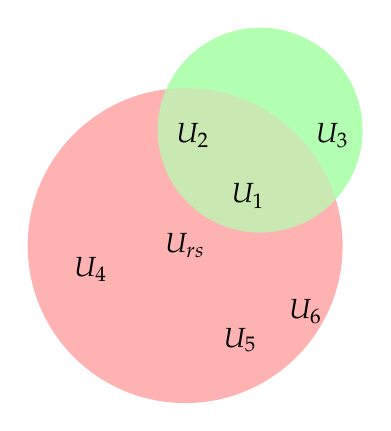
\begin{tikzpicture}
		\path[fill=red!30] (0:0cm) circle (2cm);
		\path[fill=green!30] (57:1.75cm) circle (1.3cm);

		\begin{scope}
			\clip(57:1.75cm) circle (1.3cm);
			\path[fill=red!30!green!30] (0:0cm) circle (2cm);
		\end{scope}

		\node at (0,	0) 		{$U_{\gls{rs}}$};
		\node at (0.8,	0.63) 	{$U_1$};
		\node at (0.1,	1.4)	{$U_2$};
		\node at (1.87,	1.4) 	{$U_3$};
		\node at (-1.2,	-0.3)	{$U_4$};
		\node at (0.7,	-1.2) 	{$U_5$};
		\node at (1.53, -0.84) 	{$U_6$};
	\end{tikzpicture}
	\label{fig:astepgroup}
	\caption{How the \gls{rs}-system would use \DIFdelbeginFL \DIFdelFL{gropus}\DIFdelendFL \DIFaddbeginFL \DIFaddFL{groups}\DIFaddendFL . In the red group (the red circle) all users in that group can see all data from other users in the same group.}
\end{figure}

\DIFdelbegin \paragraph{\DIFdel{Edges}} %DIFAUXCMD
\addtocounter{paragraph}{-1}%DIFAUXCMD
\DIFdel{works is }\DIFdelend \DIFaddbegin \textbf{\DIFadd{Edges}}\\ 
\DIFadd{Edges work in }\DIFaddend a similar way to groups\DIFdelbegin \DIFdel{but instead of granting all users access to every other users data, the edges only allow }\DIFdelend \DIFaddbegin \DIFadd{, but only allowing }\DIFaddend access from one user to another\DIFdelbegin \DIFdel{.
Using }\DIFdelend \DIFaddbegin \DIFadd{, corresponding to a group of two users.
This can be accomplished by establishing communication using }\DIFaddend the same method of \DIFdelbegin \DIFdel{establishing communication }\DIFdelend as with the groups \DIFdelbegin \DIFdel{we create }\DIFdelend \DIFaddbegin \DIFadd{and creating }\DIFaddend a \gls{rs} \DIFdelbegin \DIFdel{-user and creates a edge from that }\DIFdelend \DIFaddbegin \DIFadd{user and instantiate an edge from the }\gls{rs} \DIFaddend user to every user in the \gls{rs} system\DIFaddbegin \DIFadd{, illustrated in Figure \ref{fig:astepedge}}\DIFaddend .
This way\DIFdelbegin \DIFdel{it is }\DIFdelend \DIFaddbegin \DIFadd{, }\DIFaddend only when the \gls{rs} system uses its own user \DIFdelbegin \DIFdel{it is allowed to access data from the users}\DIFdelend \DIFaddbegin \DIFadd{the remaining user data can be accessed}\DIFaddend .

\begin{figure}[h]
	\centering
	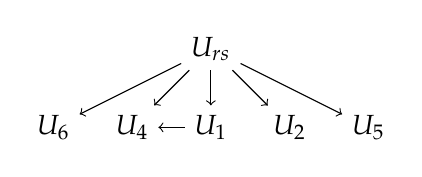
\begin{tikzpicture}

		\node (r) {$U_{\gls{rs}}$};
		\node[below of=r] (1) {$U_1$};
		\node[right of=1](2) {$U_2$};
		\node[left of=1] (4) {$U_4$};
		\node[right of=2] (5) {$U_5$};
		\node[left of=4] (6) {$U_6$};

		\draw[->] (r) -- (1);
		\draw[->] (r) -- (2);
		\draw[->] (r) -- (4);
		\draw[->] (r) -- (5);
		\draw[->] (r) -- (6);

		\draw[->] (1) -- (4);
	\end{tikzpicture}
	\DIFdelbeginFL %DIFDELCMD < \label{fig:astepgroup}
%DIFDELCMD < 	%%%
\DIFdelendFL \caption{How the \gls{rs}-system would work with edges.}
	\DIFaddbeginFL \label{fig:astepedge}
\DIFaddendFL \end{figure}

\DIFdelbegin \DIFdel{This means that edges can }\DIFdelend \DIFaddbegin \DIFadd{The edges method allows edges to }\DIFaddend provide the same \DIFdelbegin \DIFdel{benifits without opening the same security flaws.
Therefor the edges is determined to be the superior system.
}%DIFDELCMD < 

%DIFDELCMD < %%%
\DIFdel{A  overview of every API calls, as of sprint 3, required by the }%DIFDELCMD < \gls{rs}%%%
\DIFdel{-system can be seen on Table \ref{tab:asteprequests}}\DIFdelend \DIFaddbegin \DIFadd{benefits as groups while disabling the security flaw mentioned above.
Therefore, the edges method is selected as the user management design pattern}\DIFaddend .

\DIFdelbegin %DIFDELCMD < \begin{table}[h]
%DIFDELCMD < 	\centering
%DIFDELCMD < 	\scriptsize
%DIFDELCMD < 	\begin{tabular}{l l l}
%DIFDELCMD < 		%%%
\DIFdelFL{Path }%DIFDELCMD < & %%%
\DIFdelFL{Method }%DIFDELCMD < & %%%
\DIFdelFL{Description}\DIFdelendFL \DIFaddbeginFL \textbf{\DIFaddFL{Creating users}}\DIFaddendFL \\
\DIFdelbeginFL %DIFDELCMD < \midrule
%DIFDELCMD < 		%%%
\DIFdelFL{/locations/outdoor/\{username\}/routes }%DIFDELCMD < & %%%
\DIFdelFL{POST }%DIFDELCMD < & %%%
\DIFdelFL{Send a route to the }%DIFDELCMD < \gls{astep} %%%
\DIFdelFL{server}%DIFDELCMD < \\
%DIFDELCMD < 		%%%
\DIFdelFL{/locations/outdoor/\{username\}/routes/match }%DIFDELCMD < & %%%
\DIFdelFL{GET }%DIFDELCMD < & %%%
\DIFdelFL{Match all new routes}%DIFDELCMD < \\
%DIFDELCMD < 		%%%
\DIFdelFL{/users }%DIFDELCMD < & %%%
\DIFdelFL{POST }%DIFDELCMD < & %%%
\DIFdelFL{Create a new user}%DIFDELCMD < \\
%DIFDELCMD < 		%%%
\DIFdelFL{/users/\{username\}/outUsers }%DIFDELCMD < & %%%
\DIFdelFL{POST }%DIFDELCMD < & %%%
\DIFdelFL{Request a new out user}%DIFDELCMD < \\
%DIFDELCMD < 		%%%
\DIFdelFL{/users/\{username\}/outUsers/\{specifiedUsername\} }%DIFDELCMD < & %%%
\DIFdelFL{PUT }%DIFDELCMD < & %%%
\DIFdelFL{Accept out user}%DIFDELCMD < \\
%DIFDELCMD < 		%%%
\DIFdelFL{/users/\{username\}/token }%DIFDELCMD < & %%%
\DIFdelFL{GET }%DIFDELCMD < & %%%
\DIFdelFL{Get the current valid token for a user
	}%DIFDELCMD < \end{tabular}
%DIFDELCMD < 	\label{tab:asteprequests}
%DIFDELCMD < 	%%%
%DIFDELCMD < \caption{%
{%DIFAUXCMD
}
%DIFAUXCMD
%DIFDELCMD < \end{table}
%DIFDELCMD < 

%DIFDELCMD < %%%
\DIFdelend In sprint 2 it was also decided to \DIFdelbegin \DIFdel{created a user }\DIFdelend \DIFaddbegin \DIFadd{create users }\DIFaddend through the \gls{rs} server, this \DIFdelbegin \DIFdel{have }\DIFdelend \DIFaddbegin \DIFadd{has }\DIFaddend been changed to simplify the implementation \DIFdelbegin \DIFdel{.
}\DIFdelend \DIFaddbegin \DIFadd{and reduce design complexity.
}

\DIFaddend When a user registers in the \DIFdelbegin \DIFdel{app }\DIFdelend \DIFaddbegin \gls{rs} \DIFadd{app, the app will issue }\DIFaddend an API call \DIFdelbegin \DIFdel{will be issued }\DIFdelend \DIFaddbegin \DIFadd{directly }\DIFaddend to the \gls{astep} API\DIFdelbegin \DIFdel{directly from the app where before this was done }\DIFdelend \DIFaddbegin \DIFadd{, instead of performing the operation }\DIFaddend through the \gls{rs} server. 
The username and \DIFdelbegin \DIFdel{the additional information}\DIFdelend \DIFaddbegin \DIFadd{additional information, }\DIFaddend such as phone number and full name\DIFdelbegin \DIFdel{are still transfered }\DIFdelend \DIFaddbegin \DIFadd{, will still be transferred }\DIFaddend to the \gls{rs} server \DIFdelbegin \DIFdel{for storing}\DIFdelend \DIFaddbegin \DIFadd{to enable contact information sharing with other }\gls{rs} \DIFadd{users}\DIFaddend .


\subsection{Location Gathering}\DIFaddbegin \label{section:s3locgath}
\DIFaddend The location gathering should \DIFdelbegin \DIFdel{as previously discussed be performed seamlessly }\DIFdelend \DIFaddbegin \DIFadd{be performed unnoticeable }\DIFaddend for the user and in the background without any \DIFdelbegin \DIFdel{user interaction necessary }\DIFdelend \DIFaddbegin \DIFadd{necessary user interactions}\DIFaddend . 
This requires certain design \DIFdelbegin \DIFdel{requirements which }\DIFdelend \DIFaddbegin \DIFadd{features that }\DIFaddend will be presented in the following \DIFdelbegin \DIFdel{text. 
The location gathering should be a background service which will run i the background once the user have logged into the app. }\DIFdelend \DIFaddbegin \DIFadd{sections. }\DIFaddend 


\subsubsection{Overall Design}
The informal tests performed in sprint 2\DIFaddbegin \DIFadd{, Section \ref{sec:s2test}, }\DIFaddend showed that polling locations with fixed intervals controlled by a timer proved difficult to get working reliably, as the Google API client never seemed to connect before the task had finished executing. 
Thus we explore the possibility of using a broadcast receiver which does not provide fixed time intervals, but receives updates within a defined time interval.

To ensure location gathering is not performed more than necessary, the activity recognition service should be running continuously and decide the location gathering status.
The service should start requesting locations when the user is detected as driving. 
The location updates request is done through the Google Play Service location API which Google recommends above the native Android location framework \cite{apploc}.
As long as the activity registers the user as driving, the location should be received with reasonable intervals.
The gathered locations should be collected into a group of locations representing the current route.
When the the activity recognition has not been registered as driving in 5 minutes the route is considered ended, and the route building should be finalized and send to the server.

\subsubsection{Polling frequency}
The location update and activity recognition frequency is balanced between energy consumption and accuracy.

First, we consider the initial task of the location gathering service: The activity recognition.
The activity recognition is used to decide the location requests, as it has lower consumption than the GPS unit \DIFdelbegin \DIFdel{. }%DIFDELCMD < \todo{source}
%DIFDELCMD < %%%
\DIFdelend \DIFaddbegin \DIFadd{\mbox{%DIFAUXCMD
\cite{fuckGPS} }%DIFAUXCMD
since the GPS system prevents a phone form going into it's normal sleep cycles.
}\DIFaddend Many newer smartphones \DIFdelbegin %DIFDELCMD < \todo{source} %%%
\DIFdelend \DIFaddbegin \DIFadd{\mbox{%DIFAUXCMD
\cite{coCPU} }%DIFAUXCMD
}\DIFaddend have dedicated processes to track the sensors responsible for activity recognition and therefore use little power.
The interval of activity recognition will be set to \DIFdelbegin \DIFdel{a couple of }\DIFdelend \DIFaddbegin \DIFadd{every 5 }\DIFaddend seconds, which later can be optimized to use less power or be more accurate if needed.

The location request which will be called when a user is detected driving, and will in most cases need to activate a device's GPS and thus consume a lot of power.
The first iteration of location gathering it will be a simple solution which will request with static intervals, whereas dynamic intervals based on factors such as speed possibly could be evaluated for battery optimization later on.
The location updates interval will be set to \DIFdelbegin \DIFdel{range of every 1-2 minutes.
}\DIFdelend \DIFaddbegin \DIFadd{most frequently at 1 minute, but targeted at every 2 minutes.
Although the interval values are within the time scope, the values are susceptible to changes depending on test results.
}\DIFaddend 

%This will be the initial setup, if experience shows need of possible for improvements the intervals will be optimized accordingly.


\DIFdelbegin \subsection{\DIFdel{App-to-aSTEP communication}}

%DIFAUXCMD
\addtocounter{subsection}{-1}%DIFAUXCMD
%DIFDELCMD < 

%DIFDELCMD < 
%DIFDELCMD < %%%
\DIFdelend \section{Implementation}
\DIFaddbegin \DIFadd{The implementation section contains descriptions of selected parts of the implementation performed in sprint 3.
}\DIFaddend 

\DIFaddbegin \DIFadd{The main focus is the location gathering service, which will record locations continuously while the user is driving, but not otherwise. 
}

\DIFaddend \subsection{Location Gathering Background service}
% metatext
This subsection will describe the contents of the implementation of the background location gathering.
The new implementation is \DIFdelbegin \DIFdel{based }\DIFdelend \DIFaddbegin \DIFadd{founded }\DIFaddend on the poor results \DIFdelbegin %DIFDELCMD < \todo{can we document the poor results?} %%%
\DIFdelend of the location gathering method implemented in sprint 2\DIFaddbegin \DIFadd{, Section \ref{section:locationgathering}, }\DIFaddend that was not working as intended.
The code examples in this section will not include potential logging and debugging lines as \DIFdelbegin \DIFdel{to save space }\DIFdelend \DIFaddbegin \DIFadd{for better readability }\DIFaddend and they do not influence the functionality of the code.

\DIFaddbegin \textbf{\DIFadd{Implementation plan}}\\
\DIFadd{According to the design, Section \ref{section:s3locgath}, the locations should first be requested when the user is driving.
Therefore, the implementation starts by instantiating an activity detector.
The activity detector can thereafter check the received activity, and begin location gathering if the activity is above a confidence threshold for driving activity.
When the confidence is lower than the threshold for a period of time, the driving activity can be considered finished, and the route must be stored and later transmitted to the }\gls{astep} \DIFadd{system.}


\DIFaddend % activityRecognitionInstantiation
\DIFaddbegin \textbf{\DIFadd{Activity recognition instantiation}}\\
\DIFaddend The location gathering should first detect that the device is in a driving activity and then begin recording locations, according to the design described in Section \ref{ssec:LocationGatherBGS}.
To achieve the functionality, the app must connect to a Google API client and subscribe to activity recognition.
The code for subscribing to the activity recognition is shown in Listing \ref{activityRecognitionInstantiation}.
The activity recognition can thereafter check that the detected activity is a driving activity, and accordingly activate the location gathering.

\begin{lstlisting}[language=Java, label=activityRecognitionInstantiation, caption=Initialization of activity recognition.]
if(activityDetectionBroadcastReceiver == null) {
	activityDetectionBroadcastReceiver = 
		new ActivityDetectionBroadcastReceiver(googleApiClient, this);

	LocalBroadcastManager.getInstance(this).registerReceiver(
		activityDetectionBroadcastReceiver, 
		new IntentFilter("fapptory_inc.rideshare.BROADCAST_ACTION"));
}
\end{lstlisting}

The \texttt{activityDetectionBroadcastReceiver} is an instantiation of the\\ \texttt{ActivityDetectionBroadcastReceiver} class from, utilizing the \texttt{googleApiClient} and \texttt{this} which in this case references the current \texttt{MainActivity} instance to broadcast detected activities.

The broadcast receiver is then applied by registering to the \gls{rs} app's\\ \texttt{BROADCAST\_ACTION}, so that the \texttt{activityDetectionBroadcastReceiver} only handles broadcasts sent by \gls{rs} and not by other apps.

% ActivityIntentService broadcast description



% Activity Detection Broadcast Receiver
\DIFaddbegin \textbf{\DIFadd{Activity Detection Broadcast Receiver}}\\
\DIFaddend The main operations in regards to activity detection and location gathering are done by the activity detection broadcast receiver.

When the \texttt{activityDetectionBroadcastReceiver} receives a RideShare broadcast, the extra data in the broadcast is stored in the \texttt{ArrayList<DetectedActivity> detectedActivities}.
The \texttt{detectedActivities} is iterated over, shown in Listing \ref{activityRecognitionIteration} to find the driving activity \texttt{DetectedActivity.IN\_VEHICLE}.
The \texttt{startLocationUpdates()}, which is described later, is called if the confidence is above the threshold and if locations are not currently being recorded.
Line 8 controls the location cache in case a drive is stopped temporarily and starts again, appending the cached route to the actual route.

\begin{lstlisting}[language=Java, label=activityRecognitionIteration, caption=Iteration over received list of activity recognition.]
for (DetectedActivity da: detectedActivities){
	if(da.getType() == DetectedActivity.IN_VEHICLE){
		if(da.getConfidence() >= ACTIVITY_CONFIDENCE_VALUE){
			if(!isCurrentlyCollectingLocations) {
				startLocationUpdates();
				isCurrentlyCollectingLocations = true;
			}
			if(potentialStopDrivingActivity && potentialAstepRoute.size() > 0){
				astepRoute.addAll(astepRoute.size(), potentialAstepRoute);
				potentialAstepRoute.clear();
			}
			lastDetectedVehicleActivity = System.currentTimeMillis();
			potentialStopDrivingActivity = false;
			drivingActivityDetected = true;
		}
	}
}
\end{lstlisting}

% Location Updates Request
\DIFaddbegin \textbf{\DIFadd{Location Updates Request}}\\
\DIFaddend The \texttt{startLocationUpdates()}, shown in Listing \ref{startLocationUpdates}, is called to gather locations regularly.
The location updates request is based on the Google API client instantiated in \texttt{MainActivity} and a \texttt{locationRequest}.
The \texttt{locationRequest} is defined with properties regarding location update interval, fastest interval, and location \DIFdelbegin \DIFdel{quality }\DIFdelend \DIFaddbegin \DIFadd{accuracy }\DIFaddend priority, respectively set to \DIFdelbegin %DIFDELCMD < \todo{agree upon constants} %%%
\DIFdelend 60 seconds, \DIFdelbegin \DIFdel{120 }\DIFdelend \DIFaddbegin \DIFadd{60 }\DIFaddend seconds and \texttt{PRIORITY\_HIGH\_ACCURACY}.

\begin{lstlisting}[language=Java, label=startLocationUpdates, caption=Start location updates functions.]
public void startLocationUpdates(){
	if(/* Omitted: Check permissions */) {
		LocationServices.FusedLocationApi
			.requestLocationUpdates(googleApiClient, locationRequest, this);
	}
}
\end{lstlisting}

\DIFdelbegin \DIFdel{To send the routes gathered through the location service, the communication with }\DIFdelend \DIFaddbegin \subsection{\DIFadd{Route Matching Algorithm}}
\DIFadd{The implementation of the route matching algorithm is delegated to the previously mentioned outdoor location based service group, as they are responsible for implementation in the }\DIFaddend \gls{astep} \DIFdelbegin \DIFdel{must be established.
}\DIFdelend \DIFaddbegin \DIFadd{system.
They were given the pseudocode algorithm developed in sprint 2 and cooperated with during the implementation process.
The implementation will not be documented here, as the implementation is not performed by us.
However, the implementation should be tested, and we generated test data with accompanying result expectations.
The test data was also handed over, but this will be described in the following test section.}\DIFaddend 



\subsection{App-to-aSTEP communication}
%DIF <  ja..
%DIF > meta text
\DIFaddbegin \DIFadd{This section contains an overview of the implementation of the API calls utilized to communicate with }\gls{astep}\DIFadd{.}

\DIFadd{In the previous design phases it was decided what API calls should be implemented in the app.
A specified list of calls only to be performed on the app can be seen in Table \ref{tab:asteprequests}.}

\begin{table}[h]
	\centering
	\scriptsize
	\begin{tabular}{l l l}
		\DIFaddFL{Path }& \DIFaddFL{Method }& \DIFaddFL{Description}\\\midrule
		\DIFaddFL{/locations/outdoor/\{username\}/routes }& \DIFaddFL{POST }& \DIFaddFL{Send a route to the }\gls{astep} \DIFaddFL{server}\\
		\DIFaddFL{/users }& \DIFaddFL{POST }& \DIFaddFL{Create a new user}\\
		\DIFaddFL{/users/\{username\}/token }& \DIFaddFL{GET }& \DIFaddFL{Get the current valid token for a user}\\
		\DIFaddFL{/users }& \DIFaddFL{POST }& \DIFaddFL{Invalidate old token and get new}\\
		\DIFaddFL{/users/\{username\}/token }& \DIFaddFL{POST }& \DIFaddFL{Invalidates previous token for a user}\\
	\end{tabular}
	\caption{\DIFaddFL{Caption}}
	\label{tab:asteprequests}
\end{table} 

\DIFadd{The API calls are implemented using a }\texttt{\DIFadd{HttpURLConnection}} \DIFadd{class, which is a }\texttt{\DIFadd{URLConnection}} \DIFadd{class for HTTP specific data transfer over the web.
}\texttt{\DIFadd{HttpURLConnection}} \DIFadd{may be used to send and receive streaming data whose length is not known in advance.
This is needed as every API call varies in size.
E.g., the API call to post a route will be the one that varies the most in size as routes differ in size, based on the number of locations and their accuracy.}


\DIFadd{Using an object orientated structure, each API call is implemented to overwrite a }\texttt{\DIFadd{helperClass}} \DIFadd{which will handle the inputs, such as username, password, token, and routes.
The inputs are then transformed to a part of an URL which would fit each of the relevant API calls.
The }\texttt{\DIFadd{helperClass}} \DIFadd{is then parsed to the }\texttt{\DIFadd{HttpURLConnection}} \DIFadd{which will use a string builder to create the final URL from the API base URL, }\texttt{\DIFadd{http://astep.cs.aau.dk:80/api/}}\DIFadd{.
Lastly, the }\texttt{\DIFadd{HttpURLConnection}} \DIFadd{is trying to perform the API call from where response codes are handled.}

\DIFadd{It should be noted that passwords are not in the URL part of the API call, as these will be logged on the }\gls{astep} \DIFadd{server. 
This would be a major security issue.
Instead password and tokens are parsed as part of the body, which is used by REST. 
This will hide the content from the URL and instead be transfered in an }\texttt{\DIFadd{OutputStream}} \DIFadd{encoded in raw bytes. }

\DIFadd{Two examples of API calls can be seen in List \ref{list:example}.
The post route example is simplified to reduce size and make it better explainable.}

\todo{fix references and captions}

\begin{enumerate}
\label{list:example}
\item \DIFadd{POST new user
}\begin{enumerate}
\item \DIFadd{URL: http://astep.cs.aau.dk:80/api/users?username=USERNAME
}\item \DIFadd{CURL: curl -X POST --header 'Content-Type: application/json' --header}\\
 \DIFadd{'Accept: application/json' -d 'PASSWORD' 'http://astep.cs.aau.dk:80/api/users?username=USERNAME'
}\end{enumerate}
\item \DIFadd{POST route to }\gls{astep}
\begin{enumerate}
\item \DIFadd{URL: http://astep.cs.aau.dk:80/api/locations/outdoor/outdoor/routes?authorization=TOKEN\&route=longitude,latitude,precision,timestamp;\&route=longitude,latitude,precision,timestamp
\&distance\_weight\&time\_weight\&largest\_acceptable\_detour}\\
\DIFadd{\_length=146\&acceptable\'httptime\_difference=32
}\item \DIFadd{CURL: curl -X POST --header 'Content-Type: application/json' --header 'Accept: application/json' 'URL from above'
}\end{enumerate}
\end{enumerate}

\DIFadd{As seen in Create user in List \ref{list:example}, the username is parsed in the URL while the password is included in a header.
On the other hand, the post route is only parsed in the URL as there is no information that needs to be hidden.
Every decision made regarding parsing data from the apps to the }\gls{astep} \DIFadd{server is decided by the individual }\gls{astep} \DIFadd{API groups.}



\DIFaddend \section{Test}
\DIFaddbegin \DIFadd{A test of the location gathering background service was performed to examine the functionality, performance and reliability.}\DIFaddend 

\subsection{Location gathering as background service}
%DIF >  test setup
\DIFaddbegin \DIFadd{The }\gls{rs} \DIFadd{app was built and installed on three units to test on a variation of devices.
The devices were a Sony Xperia Z2, a Samsung Galaxy S6 and a Huawei Nexus 6P, all with Android Marshmallow 6.0.1 as operating system.
The app was opened and the necessary permissions were granted, so that the app could function properly.
The app was configured with the values seen in Table \ref{tab:appconfig}.}\DIFaddend 

\DIFdelbegin \subsection{\DIFdel{App-to-aSTEP communication}}

%DIFAUXCMD
\addtocounter{subsection}{-1}%DIFAUXCMD
\DIFdelend \DIFaddbegin \begin{table}[!ht]
	\centering
	\begin{tabular}{l r l}
		\DIFaddFL{Variable description }& \DIFaddFL{Value }& \DIFaddFL{Unit}\\
		\hline
		\DIFaddFL{Fastest location update interval }& \DIFaddFL{60000 }& \DIFaddFL{milliseconds}\\
		\DIFaddFL{Target location update interval }& \DIFaddFL{60000 }& \DIFaddFL{milliseconds}\\ 
		\DIFaddFL{Activity confidence value }& \DIFaddFL{80 }& \DIFaddFL{percent}\\
		\DIFaddFL{Activity stop threshold }& \DIFaddFL{180000 }& \DIFaddFL{milliseconds}\\
		\DIFaddFL{Minimum number of route locations }& \DIFaddFL{4 }& \DIFaddFL{locations }\\
		\DIFaddFL{Request activity updates }& \DIFaddFL{5000 }& \DIFaddFL{milliseconds}\\ 
	\end{tabular}
	\caption{\DIFaddFL{Parameter configuration in test of the background service route tracking.}}
	\label{tab:appconfig}
\end{table}

\DIFaddend 

%DIF >  device setup
\DIFaddbegin \iffalse
\DIFadd{To make sure the app would gather locations in different states, the phones had different configurations.
The Xperia Z2 was locked and connected to a computer for debugging purposes and logging events.
The Nexus 6P had the app open with a locked and turned off screen. 
The Galaxy S6 had the app opened, was returned to the home screen and then locked.}\todo{not sure if this paragraph is necessary}
\fi
%DIF >  route plan
\DIFadd{The route driven to test the location gathering can be seen in Figure \ref{fig:testroute}.
The route was driven with the intention of gathering the whole route as a single route on each of the devices.
The drive had one stop at the point marked by a green square in Figure \ref{fig:testroute}.
The stop had a duration of 2 minutes, thus not passing the threshold value of 3 minutes.
The drive continued and ended at the start position, where the persons of the respective devices walked from the vehicle to the group room.}

\begin{figure}[h]
	\begin{subfigure}[b]{0.55\textwidth}
		\includegraphics[width=\textwidth, trim={0 0 1cm 0},clip]{figures/testroute.png}
		\caption{\DIFaddFL{Test drive route, driven clockwise from the red pin.}}
		\label{fig:testroute}
	\end{subfigure}
	\begin{subfigure}[b]{0.44\textwidth}
		\includegraphics[width=\textwidth, trim={0 0 2cm 1.2cm},clip]{figures/testRouteRecordings.png}
		\caption{\DIFaddFL{Recorded routes. Orange route is Nexus 6P, red route is Xperia Z2 and green route is Galaxy S6.}}
		\label{fig:testrouterecordings}
	\end{subfigure}
	\caption{\DIFaddFL{Actual route and recorded route data.}}
\end{figure}

%DIF >  test results
\DIFadd{All three devices were able to gather the driven route. 
The routes were recorded with approximately the same start and end time, and the recorded routes can be seen in Figure \ref{fig:testrouterecordings}. 
As the figure shows, the gathered route data relatively accurately represent the actual route.}


\DIFadd{The Xperia device had the largest deviation from the actual route, and this could be caused by multiple factors.
Because the device was placed below the debugging laptop, interference with the GPS signals could occur.
The device could also have a poorly manufactured GPS unit.
This is not further investigated, as the two other devices gathered fairly accurate locations during the test.}



%DIF >  results evaluation
\DIFadd{The test reveals that the app is able to gather locations whilst the app is not actively being utilized by a user.
The location accuracy seems to be device specific.
Location gathering as a background service is considered accomplished and the respective requirement is evaluated as fulfilled.
}



\DIFaddend \subsection{Route Match Algorithm}
%DIF >  metatext
\DIFaddbegin \DIFadd{The route matching algorithm is implemented by one of the }\gls{astep} \DIFadd{outdoor groups, and to check that the implementation reflects the intention a test is performed.
}

\DIFadd{The implementation is tested with a sequence of routes inserted into a previous empty route database.
By adding routes sequentially, we can anticipate the matching outcome for each addition.
}


\DIFaddend % test data
\DIFaddbegin \textbf{\DIFadd{Test Data}}\\
\DIFadd{A number of cases should be tested, and we generate route data for each. 
Before the route data is input users U1, U2, U3 and U4 are created to the }\gls{astep} \DIFadd{system.}\DIFaddend 

\DIFaddbegin \DIFadd{First, the stable route generation must be confirmed functioning.
A route is created for U1 and made two copies that were slightly edited in location and time, and skewed respectively one and two weeks ahead of the original route.
These three routes should be assessed a high matching score, close to 1, and be considered a stable route for this user.
}

\DIFadd{Second, the algorithm should not be matching routes that are not relevant in location or time.
U2 gets two routes added not matching in location, as seen in Figure \ref{fig:algroutes}.
The blue U2 route is during the day time and the black during night time.
These routes should thus be assessed a low match score, assumed 0.
}

\DIFadd{Because the algorithm should match routes of different users, we thirdly created two routes for the user U3.
The routes were differencing slightly in locations and time, but were made with the intention to match with each other, with one week difference in time.
The routes were also made to roughly overlap with the routes of U1, so that U1's stable route would roughly be a sub-route of the U3 route.
}

\DIFadd{Lastly, the U4 route was made to discern location and time matching of the algorithm.
The route is stable and approximately at the same time as the U1 and U3 routes, but is directed in the opposite way, northwest instead of southeast.
The U4 route should match poorly with U1 and U3 routes, close to 0, but could score a bit higher, as the locations overlap with U3 route.
}

\begin{figure}[h]
	\centering
	\includegraphics[width=0.7\textwidth]{figures/algorithmroutes.png}
	\caption{\DIFaddFL{Generated routes to be tested by the algorithm.}}
	\label{fig:algroutes}
\end{figure}


\DIFaddend % other group executed their implemenation on test data
\DIFaddbegin \textbf{\DIFadd{Test Execution}}\\
\DIFadd{We had no influence over the actual method of the testing, but we received the following test results in Figure \ref{fig:algresults} from the outdoor group.
}\DIFaddend 


% test results
\DIFaddbegin \textbf{\DIFadd{Test Results}}\\
\DIFadd{The test results seen in Figure \ref{fig:algresults} reveal that the algorithm is performing correctly.
The results correspond to the assumptions made during the data generation.
All three routes of U1 are matched highly, as expected.
The U3 route is matching reasonably well with the U1 routes, and neither of the U1 routes are matching with the U3 route.
The results reflect that U3 can pick up U1 along the way, while U1 will have to make a significant detour to pick up U3.
}\DIFaddend 

\DIFaddbegin \begin{figure}[h]
	\centering
	\includegraphics[width=0.8\textwidth]{figures/newtestresultrs.png}
	\caption{\DIFaddFL{Results generated by the implemented algorithm.}}
	\label{fig:algresults}
\end{figure}


\DIFaddend % test results conciderations 
\DIFaddbegin \textbf{\DIFadd{Test Conclusion}}\\
\DIFadd{The algorithm test results are considered sufficient for the current application. 
However testing, including user interviews, over large amounts of data for actual users is necessary to confirm the practical convenience of the score results.
The design of the algorithm allows adjustment of several parameter concerning distance, time and the the weight of those in the final score by changing parameters in the }\gls{rs} \DIFadd{server's call to }\gls{astep} \DIFadd{system. 
}\DIFaddend 


% Sprint 4
\chapter{Sprint 4}
%meta - to edit
Sprint four is the fourth and last iteration of the project.

\section{Analysis}

\subsection{Missing features for completing the solution}

\subsection{Algorithm results analysis}


% Sprint 4 krav
\subsection{Requirements for the fourth sprint}


% something
\textbf{Route Matching Algorithm}\\
placeholder


\section{Design}
% metatext


\subsection{Algorithm redesign}


\subsection{Algorithm test design}



\subsection{RideShare Server Design}


\section{Implementation}

\subsection{RideShare Server}
% indhold i server



% kommunikation med aSTEP



% respons/kommunikation med app
\section{Test}
% metatext for test section


\subsection{Background location gathering}


\subsection{RideShare Server}


\subsection{App-RideShare Server Communication}


\subsection{App-aSTEP Communication}


\subsection{RideShare Server-aSTEP Communication}


\subsection{App-RideShare Server Communication}



% Summary
\chapter{Summary}
\section{Reflection}
Some to come here
\section{Conclusion}
I made dis.
\section{Future Work}
Fix it.

% Bibliography
\printbibliography[heading=bibintoc]
\label{bib:mybiblio}

% Appendix
\appendix
\chapter{Sprint 3 API functionality}\label{ch:appAlabel}
\DIFdelbegin \DIFdel{Here is the first appendix}\DIFdelend \DIFaddbegin \DIFadd{In the following table are the API functionality as they were in sprint 3 with regards to UM and outdoor location based service.
Indoor location based service is omitted. The list is based on the information available at }\url{http://www.astep.cs.aau.dk/}\DIFadd{.
At the URL the most recent version of the API will be available at any given time.
}

\begin{table}[!ht]
	\centering
	\begin{tabular}{ll}
		\DIFaddFL{Outdoor location services }& \DIFaddFL{User Management    }\\
		\hline
		\begin{tabular}[t]{@{}l@{}}
			\DIFaddFL{Get user past location}\\ \DIFaddFL{Get user past locations area}\\ \DIFaddFL{Get user past Locations radius}\\ \DIFaddFL{post user current location}\\ \DIFaddFL{Post user current route}\\ \DIFaddFL{Get all new route matches}\\ \DIFaddFL{Get all locations friends}\\ \DIFaddFL{Get all users in area }\\ \DIFaddFL{Get locations friends }\\ \DIFaddFL{Get subset of users area }\\ \DIFaddFL{Get users outside area }\\\DIFaddFL{Get subset of users radius }\\ \DIFaddFL{Get locations friend timestamp}\end{tabular}
		&
		\begin{tabular}[t]{@{}l@{}}
			\DIFaddFL{Create group }\\ \DIFaddFL{Get administrated groups}\\ \DIFaddFL{Add administration}\\ \DIFaddFL{Remove administration }\\ \DIFaddFL{Get invited users }\\ \DIFaddFL{Invite user to group }\\ \DIFaddFL{Revoke group invitation }\\ \DIFaddFL{Get members of a group }\\ \DIFaddFL{Remove user from group }\\ \DIFaddFL{Create user }\\ \DIFaddFL{Get groups that a user is invited to }\\ \DIFaddFL{Decline group invitation }\\ \DIFaddFL{Get groups that user is member of }\\ \DIFaddFL{Join group }\\ \DIFaddFL{Leave group }\\ \DIFaddFL{Get outdoor-user}\\ \DIFaddFL{Request outdoor user }\\ \DIFaddFL{Delete outdoor-user }\\ \DIFaddFL{Validate outdoor-user}\\ \DIFaddFL{Change password}\\ \DIFaddFL{Get token }\\ \DIFaddFL{Issue token}\end{tabular}
	\end{tabular}
	\caption{\DIFaddFL{Currently planned aSTEP API functions.}}
	\label{tbl:s3api}
\end{table}
 \DIFaddend\end{document}